\documentclass[12pt,a4paper]{report}
\usepackage{titlesec}
\usepackage{graphicx}
\usepackage{amsmath}
\usepackage{booktabs}
\usepackage{float}
\usepackage[utf8]{inputenc}
\usepackage[T1]{fontenc}
\usepackage{lmodern}
\usepackage{setspace}
\usepackage{geometry}
\PassOptionsToPackage{hyphens}{url}
\usepackage[hidelinks]{hyperref}
\usepackage{enumitem}
\usepackage{fancyhdr}
\usepackage{url}
\usepackage[font=small, skip=6pt]{caption}

% Tighter float spacing for improved page utilisation
\setlength{\floatsep}{8pt plus 2pt minus 2pt}
\setlength{\textfloatsep}{10pt plus 2pt minus 4pt}
\setlength{\intextsep}{8pt plus 2pt minus 2pt}
\emergencystretch=2em

\pagestyle{fancy}
\fancyhf{}
\fancyhead[L]{Chapter \thechapter: \nouppercase{\leftmark}}
\renewcommand{\chaptermark}[1]{\markboth{#1}{}}
\fancyhead[R]{\thepage}
\renewcommand{\headrulewidth}{0.2pt}

\geometry{margin=1in, headheight=15pt}
\onehalfspacing
\setlist[itemize]{noitemsep, topsep=4pt}

\titleformat{\chapter}[display]
{\normalfont}
{\Huge\bfseries Chapter \thechapter}{10pt}
{\Huge\bfseries}

\begin{document}

\newpage

\chapter*{Abstract}
\addcontentsline{toc}{chapter}{Abstract}

Crop diseases cause yield losses of 20--40\% annually, disproportionately affecting smallholder farmers who lack timely diagnostic expertise~\cite{b8}. Most existing deep-learning-based detection systems stop at classification without providing actionable remediation guidance, limiting their practical utility in the field.

This work presents \textbf{Deep Learning-Based Plant Disease Detection for Cotton and Wheat with Context-Aware Remediation Advice}, integrating: (i)~a leakage-safe EfficientNetV2-S~\cite{b1} classifier with crop-specific heads for cotton (8~classes, 96.0\% accuracy) and wheat (9~classes, 92.9\% accuracy), trained with focal loss~\cite{b2}, label smoothing, and test-time augmentation; (ii)~a rule-based recommendation engine mapping each detected disease to growth-stage-specific, severity-aware remedies from ICAR, CIMMYT, and FAO; and (iii)~a GPT-4o-mini advisory layer that synthesises rule-based output into farmer-friendly guidance covering disease explanation, remedy rationale, application instructions, and itemised cost analysis at Indian market rates. Cotton and wheat were selected for their complementary importance in Indian agriculture---cotton as a major cash crop, wheat as a staple food crop---both exhibiting visually distinguishable foliar symptoms suited to image-based detection. Focusing on two crops within a minor project scope enabled rigorous dataset curation and evaluation; the modular design permits extension to additional crops by adding new classification heads and knowledge-base entries.

The system is deployed as a responsive web application backed by a FastAPI inference server and evaluated on rigorously deduplicated, group-aware dataset splits that prevent train--test contamination. Grad-CAM~\cite{b3} visualisations confirm that predictions are grounded in biologically relevant leaf regions. The proposed system demonstrates that coupling accurate detection with context-aware remediation advice produces a practical, end-to-end decision-support tool for sustainable crop protection.

\setcounter{tocdepth}{2}
\tableofcontents
\thispagestyle{plain}

\listoffigures
\addcontentsline{toc}{chapter}{List of Figures}
\listoftables
\addcontentsline{toc}{chapter}{List of Tables}
\newpage

%% =========================================================================
\chapter{Introduction}
%% =========================================================================

\section{Background and Motivation}
Agriculture remains the primary livelihood for over 58\% of India's population, and the sector contributes approximately 18\% of the national GDP~\cite{b8}. Among the many biotic stresses that threaten crop productivity, fungal, bacterial, and viral diseases collectively account for estimated yield losses of 20--40\% worldwide each year~\cite{b8,b9}. Cotton and wheat---two crops of enormous economic importance to Indian agriculture---are particularly susceptible to a wide range of foliar diseases whose visual symptoms are often subtle, overlapping, and easily confused by non-expert observers.

Traditional disease management relies on manual scouting by trained agronomists or extension workers, a process that is slow, subjective, and unavailable at scale in rural settings. Farmers frequently resort to calendar-based or prophylactic pesticide application, leading to excessive chemical use, increased production costs, environmental degradation, and the emergence of resistant pathogen strains~\cite{b10}. The advent of smartphone-based imaging and deep learning offers a compelling alternative: automated, real-time disease screening from a single leaf photograph~\cite{b7,b5}.

However, two critical gaps persist in the current landscape of AI-driven crop disease management. First, many published detection systems are evaluated on datasets with inadequate split discipline---duplicate images, near-duplicates, and source-group leakage inflate reported accuracies and erode trust in the results~\cite{b6}. Second, even well-performing classifiers typically stop at returning a disease label and a confidence score, leaving the farmer without actionable guidance on \textit{what to do next}: which chemical to apply, at what dose, at what growth stage, and at what cost~\cite{b11,b19}.

This work addresses both gaps by presenting an integrated system that combines leakage-safe disease detection with a two-tier remediation advisory module, producing a complete decision-support pipeline from image capture to treatment recommendation.

\section{Problem Statement}
The central problem addressed in this work is as follows: \textit{given a photograph of a diseased crop leaf, automatically identify the disease with high reliability and generate contextualised, actionable remediation advice tailored to the crop's growth stage, disease severity, and the farmer's operational scale.}

This problem decomposes into three sub-problems:
\begin{enumerate}
    \item \textbf{Reliable disease classification} under real-world field variability, class imbalance, and dataset quality challenges.
    \item \textbf{Evidence-based remedy selection} that accounts for growth-stage constraints and severity escalation, drawing from authoritative agricultural knowledge sources.
    \item \textbf{Farmer-friendly advisory generation} that translates technical remediation data into clear, localised guidance including application procedures, safety precautions, and cost estimates.
\end{enumerate}

\section{Main Contributions}
The main contributions of this work are as follows:
\begin{itemize}
    \item A unified, leakage-safe image classification pipeline instantiated for cotton (8~classes) and wheat (9~classes) using a shared EfficientNetV2-S backbone~\cite{b1} with crop-specific classification heads, trained with focal loss~\cite{b2}, label smoothing, and test-time augmentation.
    \item A disciplined dataset engineering methodology employing SHA-256 exact-duplicate removal, perceptual-hash near-duplicate filtering, cross-class ambiguity elimination, and source-group-aware split enforcement to guarantee zero train--test contamination.
    \item A two-tier remediation advisory module comprising a rule-based recommendation engine (sourced from ICAR, CIMMYT, FAO, and other institutional authorities) and a GPT-4o-mini-powered LLM advisory layer that generates structured, farmer-friendly guidance with Indian market cost estimates.
    \item An end-to-end web-based deployment (FastAPI backend, React frontend) with Grad-CAM~\cite{b3} explainability, enabling transparent and trustworthy field-level decision support.
\end{itemize}

\section{Scope and Delimitation}
The system is instantiated for two crops---cotton and wheat---which were selected for their complementary importance in Indian agriculture: wheat is a principal food crop essential for national food security, while cotton is a leading cash crop supporting millions of farming households. Both crops are affected by multiple diseases with visually distinctive foliar symptoms, making them well-suited for image-based detection and remediation advisory. Focusing the study on two crops rather than a broader set ensures controlled experimentation, eliminates cross-crop class ambiguity, and permits rigorous evaluation of every pipeline component---a priority given the scope of a minor project. The framework is, however, architecturally extensible: adding a new crop requires only a new classification head, a corresponding knowledge-base module, and growth-stage definitions; the backbone, training recipe, and advisory pipeline remain unchanged. The remediation advisory is designed for Indian agronomic conditions and market pricing; adaptation to other geographies would require updating the knowledge base and cost tables.

\section{Report Organisation}
The remainder of this report is organised as follows. Chapter~2 reviews related work in deep-learning-based plant disease detection, transfer learning for agriculture, decision support systems, and the emerging role of large language models in agricultural advisory. Chapter~3 details the system design and methodology, covering the overall system architecture, the detection pipeline, dataset engineering, model architecture, data augmentation, the rule-based recommendation engine, and the LLM advisory layer. Chapter~4 presents the experimental setup, results, ablation studies, explainability analysis, and deployment architecture. Chapter~5 concludes the report with a discussion of limitations and directions for future work.

%% =========================================================================
\chapter{Literature Review}
%% =========================================================================

\section{Deep Learning for Plant Disease Detection}
The application of deep learning to plant disease recognition has grown rapidly since the seminal work of Mohanty et al.~\cite{b7}, who demonstrated that convolutional neural networks (CNNs) trained on the PlantVillage dataset could classify 26~diseases across 14~crop species with accuracies exceeding 99\% under controlled conditions. Ferentinos~\cite{b5} extended this line of work by evaluating multiple CNN architectures---including VGG, ResNet, and Inception---on 87,848 images spanning 58~disease--plant combinations, achieving 99.53\% accuracy on the held-out test set. While these results were encouraging, subsequent studies noted that laboratory-quality images and random train--test splits contributed to overly optimistic performance estimates~\cite{b16,b6}.

Sladojevi\'{c} et al.~\cite{b6} were among the first to highlight that recognition performance degrades substantially when models trained on curated datasets are deployed on field-captured images with variable lighting, occlusion, and background clutter. Sharma et al.~\cite{b21} further demonstrated that CNN-based disease detection benefits from careful image segmentation and preprocessing to isolate symptomatic regions. More recent work by Kamilaris and Prenafeta-Bold\'{u}~\cite{b9} surveyed 40 deep-learning studies in agriculture and concluded that while CNNs consistently outperform handcrafted-feature baselines, challenges related to data quality, class imbalance, and domain shift remain prevalent.

\section{Transfer Learning and EfficientNet Architectures}
Transfer learning---fine-tuning a model pretrained on a large-scale dataset such as ImageNet~\cite{b15}---has become the dominant paradigm in agricultural image classification, significantly reducing data requirements and training time~\cite{b17}. Among modern architectures, the EfficientNet family introduced by Tan and Le~\cite{b1} has attracted particular attention due to its compound scaling strategy that jointly optimises depth, width, and resolution for superior accuracy--efficiency trade-offs.

Atila et al.~\cite{b4} applied EfficientNet-B0 through B5 to plant leaf disease classification and reported up to 99.91\% accuracy on PlantVillage, outperforming VGG16, InceptionV3, and ResNet50. Nigam et al.~\cite{b12} proposed an EfficientNet-based model specifically for wheat rust identification, demonstrating that transfer learning from ImageNet provides robust feature representations for cereal diseases. Devi and Kumar~\cite{b13} evaluated EfficientNetV2 for simultaneous plant disease and pest classification, confirming the architecture's effectiveness across diverse agricultural visual tasks. Hassan et al.~\cite{b14} conducted a comprehensive comparison of EfficientNet against six other transfer-learning architectures and found that EfficientNet models achieved the highest classification accuracy with fewer trainable parameters.

The EfficientNetV2 family~\cite{b1}, which introduced Fused-MBConv blocks and progressive learning strategies, further improved training speed by up to 6.8$\times$ while maintaining state-of-the-art accuracy. This efficiency makes EfficientNetV2-S particularly attractive for agricultural deployments where computational resources may be limited.

\section{Handling Class Imbalance and Training Robustness}
Agricultural datasets frequently exhibit class imbalance, where common diseases or healthy samples dominate while rare conditions are underrepresented. Standard cross-entropy loss can bias the model toward majority classes, reducing recall on critical minority diseases. Lin et al.~\cite{b2} introduced focal loss, which down-weights well-classified examples and concentrates learning on hard, misclassified samples. Originally proposed for dense object detection, focal loss has since been widely adopted in imbalanced classification tasks, including plant disease recognition.

Complementary regularisation techniques---label smoothing~\cite{b18}, mixup~\cite{b22}, dropout, and curriculum learning~\cite{b23}---further improve generalisation by preventing overconfident predictions and encouraging smoother decision boundaries. Data augmentation, comprehensively surveyed by Shorten and Khoshgoftaar~\cite{b17}, remains indispensable for expanding the effective training distribution, particularly for underrepresented classes captured under limited field conditions.

\section{Decision Support Systems in Agriculture}
The vision of integrating disease detection with management advice dates back to early agricultural decision support systems (DSS). Shtienberg~\cite{b19} reviewed decades of crop-protection DSS development and identified a persistent ``implementation gap'': while many systems demonstrated technical merit, adoption by farmers remained low due to complexity, lack of localisation, and disconnection from the diagnostic workflow.

Kukar et al.~\cite{b20} presented AgroDSS, a modular decision-support framework for farm management that integrated weather data, soil sensors, and crop models. Their work highlighted the importance of presenting actionable, context-specific recommendations rather than generic advice. Audsley et al.~\cite{b24} developed a foliar disease model for wheat that linked disease severity to growth-stage-specific fungicide timing, demonstrating that decision support must be temporally and agronomically contextualised to be effective.

More recently, the convergence of AI-based detection and advisory systems has been recognised as a critical frontier. However, most published plant disease detection systems still terminate at the classification output and do not incorporate the recommendation layer needed for practical field deployment~\cite{b9,b19}.

\section{Large Language Models in Agricultural Advisory}
The emergence of large language models (LLMs) has opened new possibilities for generating natural-language agricultural advice at scale. Tzachor et al.~\cite{b10} explored the potential of LLMs for agricultural extension services and noted their ability to synthesise domain knowledge into accessible, farmer-friendly guidance. Yuan et al.~\cite{b25} proposed PestGPT, a system leveraging LLMs and IoT for customised pest management recommendations, demonstrating that LLM-generated advice can be contextualised to regional conditions and crop-specific requirements.

These studies suggest that LLMs can serve as an effective interface layer between structured agricultural knowledge bases and end users, provided that the underlying factual content is grounded in authoritative sources rather than relying solely on the model's parametric knowledge. The present work adopts this grounded approach by supplying the LLM with rule-based recommendations sourced from institutional authorities, thereby constraining its output to evidence-based guidance.

\section{Explainability and Trust in Agricultural AI}
Farmer adoption of AI-based tools depends critically on trust, which in turn requires transparency in model decision-making. Selvaraju et al.~\cite{b3} introduced Gradient-weighted Class Activation Mapping (Grad-CAM), a post-hoc explainability technique that produces visual heatmaps highlighting the image regions most influential in the model's prediction. In agricultural contexts, Grad-CAM visualisations can confirm that the classifier attends to disease-relevant leaf regions---such as lesions, discolouration, and necrotic patches---rather than background artefacts or imaging conditions, thereby increasing trust and interpretability~\cite{b4,b12}.

\section{Datasets for Cotton and Wheat Disease Classification}
The proposed system is evaluated on publicly available datasets for cotton and wheat disease classification, providing diverse field-level images under varying environmental conditions. In both cases, only those images relevant to the Indian agricultural context were selected from the source repositories for use in this project.

\textbf{Cotton Dataset.} The cotton disease dataset is compiled from publicly available sources, including the Mendeley Data repository and Kaggle. It comprises 8\,750 annotated images across 8 disease and condition categories, captured under real-world field variations in lighting, occlusion, and background noise. Table~\ref{tab:cotton-raw} presents the per-class image distribution.
\begin{itemize}
    \item Source~1: \url{https://data.mendeley.com/datasets/b3jy2p6k8w/2}
    \item Source~2: \url{https://www.kaggle.com/datasets/seroshkarim/cotton-leaf-disease-dataset}
\end{itemize}

\begin{table}[H]
\centering
\caption{Cotton Dataset -- Raw Per-Class Image Distribution}
\label{tab:cotton-raw}
\begin{tabular}{lr}
\toprule
Disease Class & Images \\
\midrule
Bacterial Blight & 1\,000 \\
Leaf Curl Virus & 1\,000 \\
Herbicide Growth Damage & 1\,000 \\
Leaf Hopper (Jassid) Damage & 1\,000 \\
Leaf Reddening & 1\,000 \\
Leaf Variegation & 1\,000 \\
Healthy Leaves & 1\,000 \\
Fusarium Wilt & 1\,750 \\
\midrule
\textbf{Total} & \textbf{8\,750} \\
\bottomrule
\end{tabular}
\end{table}

\textbf{Wheat Dataset.} The wheat disease dataset is compiled from publicly available sources, including Mendeley Data and Kaggle. It comprises 13\,475 images across 9 disease and condition classes, covering rusts, blights, powdery mildew, and other wheat pathologies. As with the cotton dataset, only those images pertinent to Indian agronomic conditions were retained. Table~\ref{tab:wheat-raw} presents the per-class image distribution.
\begin{itemize}
    \item Source~1: \url{https://data.mendeley.com/datasets/5gc7hwydwg/1}
    \item Source~2: \url{https://www.kaggle.com/datasets/freedomfighter1290/wheat-disease}
\end{itemize}

\begin{table}[H]
\centering
\caption{Wheat Dataset -- Raw Per-Class Image Distribution}
\label{tab:wheat-raw}
\begin{tabular}{lr}
\toprule
Disease Class & Images \\
\midrule
Black Rust (Stem Rust) & 1\,743 \\
Black Point & 1\,000 \\
Fusarium Foot Rot & 1\,000 \\
Leaf Blight & 1\,000 \\
Powdery Mildew & 1\,151 \\
Smut & 1\,139 \\
Wheat Blast & 1\,468 \\
Yellow Rust (Stripe Rust) & 2\,974 \\
Healthy Plant & 2\,000 \\
\midrule
\textbf{Total} & \textbf{13\,475} \\
\bottomrule
\end{tabular}
\end{table}

Both datasets are preprocessed using the leakage-safe pipeline described in Chapter~3, which includes duplicate removal, near-duplicate filtering, group-aware splitting, and validation auditing to prevent data contamination and ensure reliable evaluation.

%% =========================================================================
\chapter{System Design and Methodology}
%% =========================================================================

\section{System Overview}
The proposed system is an integrated pipeline that accepts a crop leaf image as input and produces both a disease diagnosis and a comprehensive remediation advisory as output. The architecture comprises three tightly coupled modules:

\begin{enumerate}
    \item \textbf{Disease Detection Module:} A leakage-safe EfficientNetV2-S-based image classifier with crop-specific heads for cotton (8~classes) and wheat (9~classes).
    \item \textbf{Rule-Based Recommendation Engine:} A structured knowledge base that maps each detected disease to growth-stage-specific, severity-aware remedies sourced from ICAR, CIMMYT, FAO, and other institutional authorities.
    \item \textbf{LLM Advisory Layer:} A GPT-4o-mini-powered module that synthesises the rule-based output into a four-section farmer-friendly advisory covering disease explanation, remedy rationale, application guide, and cost analysis.
\end{enumerate}

The end-to-end workflow is:
\begin{center}
\textbf{Image Capture $\rightarrow$ Preprocessing $\rightarrow$ Disease Classification $\rightarrow$ Rule-Based Recommendation $\rightarrow$ LLM Advisory Generation $\rightarrow$ Farmer Dashboard}
\end{center}

This design ensures that the detection module provides high-confidence disease labels, the recommendation engine contributes evidence-based treatment data, and the LLM layer translates technical content into accessible guidance---each module compensating for the limitations of the others.

Figure~\ref{fig:system-architecture} presents the complete system architecture, illustrating the end-to-end data flow from user input to advisory output. The workflow proceeds as follows. The farmer uploads a leaf photograph through the web application frontend and provides contextual metadata---crop type, observed growth stage, perceived severity level, and farm size in acres. The \textbf{Disease Detection} module processes the image through the appropriate crop-specific EfficientNetV2-S classifier, producing a disease prediction with an associated confidence score.

The prediction, together with the user-supplied metadata, is routed to the \textbf{Recommendation Orchestrator}, a FastAPI-hosted backend that coordinates the advisory pipeline through four sequential stages. First, the \textbf{Input Validator} verifies that the declared crop is supported, that the predicted disease belongs to the specified crop's disease catalogue, and that the growth stage, severity level, and farm size fall within acceptable ranges. Second, the \textbf{Rule-Based Knowledge Engine} retrieves disease-specific information from the structured knowledge base, including disease metadata, base remedies, growth-stage-specific treatments, severity-escalated protocols, preventive measures, and source citations from authoritative institutions. Third, the \textbf{Remedy Merger and Prioritiser} deduplicates overlapping recommendations across base, stage-specific, and severity-specific entries, and ranks them by treatment priority. Fourth, the \textbf{Cost Estimation Engine} performs market-rate lookups for recommended products, computes per-acre dosages, and generates option-wise total cost breakdowns scaled to the farmer's declared acreage.

The consolidated remedy data and cost estimates are then passed to the \textbf{LLM Advisory Layer}, which employs a constrained GPT-4o-mini prompt to synthesise the structured inputs into a farmer-friendly advisory comprising four sections: disease explanation, remedy explanation, application guide, and cost analysis. The advisory is returned as a grounded JSON response, ensuring that all factual content is anchored in the rule-based output and the predefined market-rate dictionary. Finally, the \textbf{Web Application Frontend} renders the results through dedicated visual components, presenting the diagnosis alongside treatment recommendations, an application timeline, and an itemised cost comparison to support informed decision-making.

\begin{figure}[H]
\centering
\IfFileExists{full_architecture.png}{\includegraphics[width=\textwidth, height=0.42\textheight, keepaspectratio]{full_architecture.png}}{\fbox{\parbox[c][6cm][c]{\textwidth}{full\_architecture.png not available}}}
\caption[Complete system architecture of the disease detection and remediation advisory system]{Complete system architecture of the proposed Deep Learning-Based Plant Disease Detection for Cotton and Wheat with Context-Aware Remediation Advice. The diagram illustrates the end-to-end pipeline from disease detection through the recommendation orchestrator---comprising input validation, rule-based knowledge retrieval, remedy prioritisation, cost estimation, and LLM-powered advisory generation---to the farmer-facing web application interface.}
\label{fig:system-architecture}
\end{figure}

\section{Disease Detection Module}

\subsection{Dataset Engineering and Leakage Prevention}
The reliability of any supervised classification system depends fundamentally on the quality and integrity of its training data. A key contribution of this work is a disciplined dataset engineering pipeline applied uniformly to both crop domains.

\paragraph{Duplicate and Near-Duplicate Removal.}
Raw datasets frequently contain exact duplicates (identical byte-level copies) and near-duplicates (visually indistinguishable images differing only in compression or minor cropping). SHA-256 cryptographic hashes are computed for every image to identify and remove exact duplicates. For near-duplicate detection, perceptual hashing (pHash) is applied with a Hamming distance threshold, eliminating images that are visually identical but differ at the byte level.

\paragraph{Cross-Class Ambiguity Removal.}
Identical or near-identical images appearing under different class labels introduce label noise that degrades both training and evaluation. All cross-class duplicates are identified via hash comparison and removed to ensure consistent labelling.

\paragraph{Source-Group-Aware Split Enforcement.}
To prevent data leakage, splitting is performed at the source-group level rather than the individual-image level, ensuring that images from the same capture session, plant, or photographer do not appear in both training and test sets. This guarantees that reported performance reflects true generalisation rather than memorisation of correlated samples.

\paragraph{Split Auditing.}
After splitting, a post-hoc audit verifies zero hash overlap between the training, validation, and test partitions, and the split manifest is recorded for reproducibility.

\begin{table}[H]
\centering
\caption{Dataset Summary After Leakage-Safe Cleaning}
\label{tab:dataset-summary}
\begin{tabular}{lccc}
\toprule
Crop & Raw Images & Cleaned Images & Disease Classes \\
\midrule
Cotton & 8\,750 & 4\,707 & 8 \\
Wheat & 13\,475 & 9\,310 & 9 \\
\bottomrule
\end{tabular}
\end{table}

\textbf{Cotton classes (8):} Bacterial Blight, Leaf Curl Virus, Fusarium Wilt, Healthy Leaves, Herbicide Growth Damage, Leaf Hopper (Jassid) Damage, Leaf Reddening, and Leaf Variegation.

\textbf{Wheat classes (9):} Black Rust (Stem Rust), Black Point, Fusarium Foot Rot, Healthy Plant, Leaf Blight, Powdery Mildew, Smut, Wheat Blast, and Yellow Rust (Stripe Rust).

Understanding the characteristic visual symptoms of each disease class is essential for interpreting model predictions and assessing classification difficulty. Tables~\ref{tab:cotton-symptoms} and~\ref{tab:wheat-symptoms} summarise the validated diagnostic symptoms for the cotton and wheat disease classes, respectively.

\begin{table}[H]
\centering
\caption{Characteristic Symptoms of Cotton Diseases}
\label{tab:cotton-symptoms}
\begin{tabular}{lp{9.5cm}}
\toprule
Disease & Validated Characteristic Symptoms \\
\midrule
Bacterial Blight & Small water-soaked leaf spots appear first; they become angular because they are limited by veins and later turn brown to black~\cite{b26}. \\
Leaf Curl Virus & Young leaves show upward or downward curling, often with vein thickening or darkening and cup-shaped enations on the underside~\cite{b27}. \\
Herbicide Growth Damage & Leaves may become twisted, narrow, cupped, curled, or otherwise malformed; stunting and chlorosis can also occur~\cite{b28}. \\
Leaf Hopper (Jassid) Damage & Yellowing starts at leaf margins, followed by curling, reddening or bronzing, and later browning or drying (``hopperburn'')~\cite{b29}. \\
Leaf Reddening & Leaves develop reddish or purplish discolouration, usually beginning at the margins and later spreading over more of the blade~\cite{b30}. \\
Leaf Variegation & Irregular green--yellow to white--yellow patchy discolouration produces a mottled or mosaic-like appearance on leaves~\cite{b31}. \\
Healthy Leaves & No visible disease symptoms. \\
Fusarium Wilt & Yellowing usually begins on lower or older leaves, followed by drooping, wilting, and vascular browning in affected plants~\cite{b32}. \\
\bottomrule
\end{tabular}
\end{table}

\begin{table}[H]
\centering
\caption{Characteristic Symptoms of Wheat Diseases}
\label{tab:wheat-symptoms}
\begin{tabular}{lp{9.5cm}}
\toprule
Disease & Validated Characteristic Symptoms \\
\midrule
Black Rust (Stem Rust) & Dark reddish-brown rust pustules appear mainly on stems and leaf sheaths; in later stages, pustules turn black~\cite{b33}. \\
Black Point & Dark brown to black discolouration develops at the embryo (germ) end of the grain, sometimes extending to nearby grain tissue~\cite{b34}. \\
Fusarium Foot Rot & Browning and rotting occur in roots, crown, and stem base, often with dark brown lesions near the lower nodes~\cite{b35}. \\
Leaf Blight & Reddish-brown to brown lesions form on leaves, often with yellow margins; lesions may enlarge, merge, and dry the leaf~\cite{b36}. \\
Powdery Mildew & White to grey powdery fungal growth appears on leaves and may also spread to sheaths and stems~\cite{b37}. \\
Smut & Black powdery spore masses replace normal grain or floral tissues in the ear or head~\cite{b38}. \\
Wheat Blast & Partial or complete bleaching of spikelets or spikes is typical; grains may become shrivelled, poorly filled, or absent~\cite{b39}. \\
Yellow Rust (Stripe Rust) & Yellow to orange-yellow pustules form in narrow stripes along the leaves; lesions may also occur on sheaths and glumes~\cite{b40}. \\
Healthy Plant & No visible disease symptoms. \\
\bottomrule
\end{tabular}
\end{table}

\subsection{Model Architecture}
The shared backbone is EfficientNetV2-S~\cite{b1}, selected for its superior accuracy-to-efficiency trade-off achieved through Fused-MBConv blocks and progressive learning. The model accepts input images of size $224 \times 224 \times 3$. A compact classification head is attached after global average pooling:

\begin{itemize}
    \item EfficientNetV2-S backbone pretrained on ImageNet~\cite{b15}
    \item Global average pooling
    \item Batch normalisation
    \item Dropout (crop-specific: $p = 0.30$ for cotton, $p = 0.45$ for wheat) for regularisation
    \item Dense layer with crop-specific softmax activation (8~units for cotton, 9~units for wheat)
\end{itemize}

The backbone weights are initially frozen during head training and selectively unfrozen during fine-tuning, following a staged transfer-learning strategy.

\begin{figure}[H]
\centering
\begin{minipage}[t]{0.48\textwidth}
    \centering
    \IfFileExists{cotton_model_architecture.png}
        {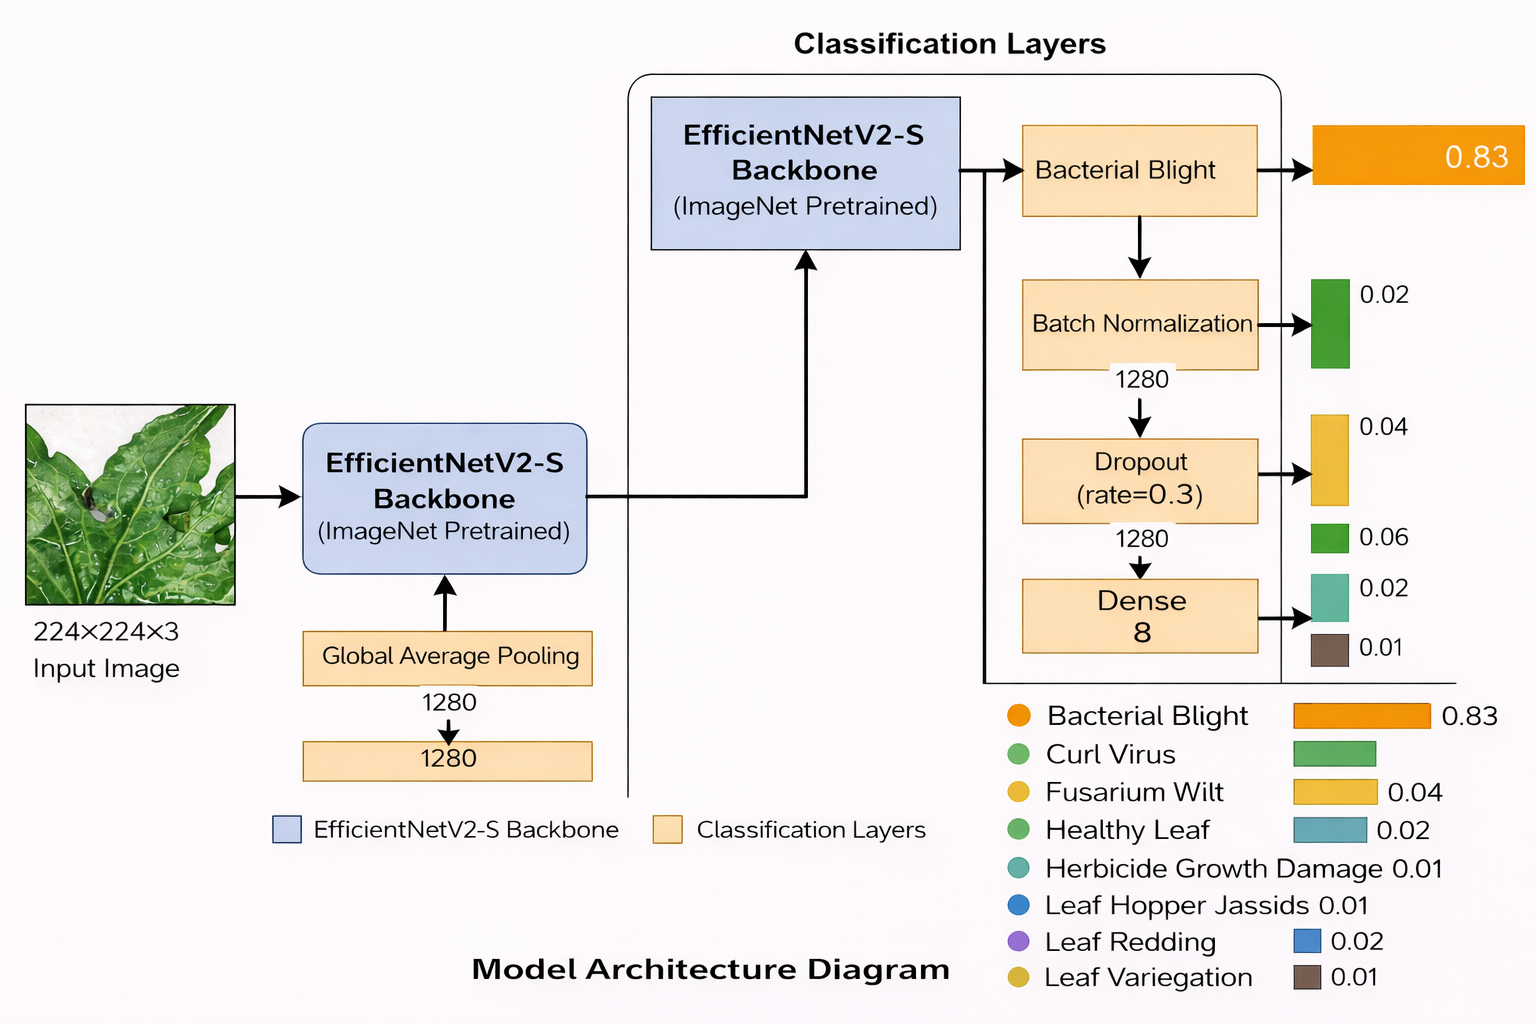
\includegraphics[width=\linewidth, height=8cm, keepaspectratio]{cotton_model_architecture.png}}
        {\fbox{\parbox[c][3cm][c]{0.95\linewidth}{cotton\_model\_architecture.png not available}}}
\end{minipage}
\hfill
\begin{minipage}[t]{0.48\textwidth}
    \centering
    \IfFileExists{wheat_model_architecture.png}
        {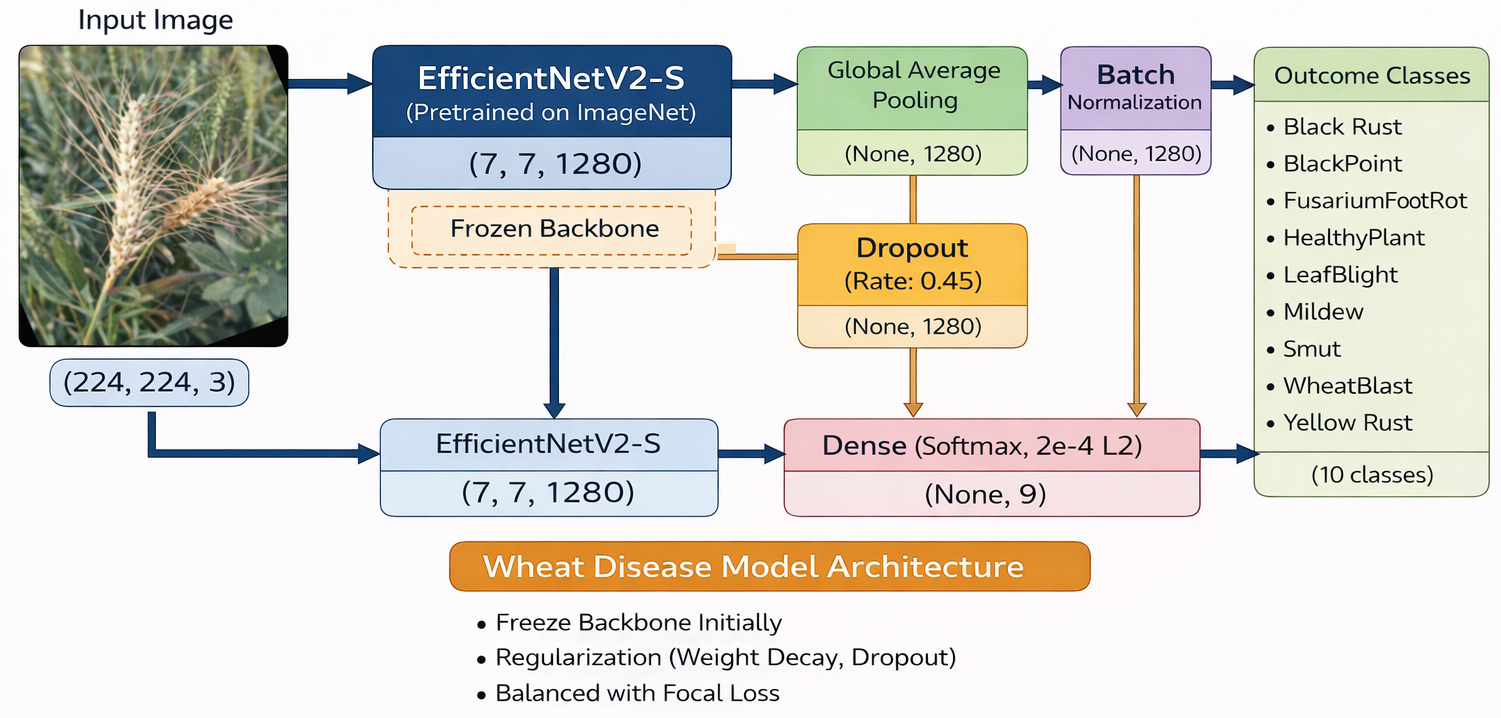
\includegraphics[width=\linewidth, height=8cm, keepaspectratio]{wheat_model_architecture.png}}
        {\fbox{\parbox[c][3cm][c]{0.95\linewidth}{wheat\_model\_architecture.png not available}}}
\end{minipage}
\caption[Crop-specific EfficientNetV2-S classification architectures for cotton and wheat]{Disease detection architectures for cotton (left, 8-class head) and wheat (right, 9-class head), both sharing the EfficientNetV2-S backbone with crop-specific classification heads.}
\label{fig:model-architectures}
\end{figure}

\subsection{Loss Function and Regularisation}
To address class imbalance and improve learning on hard examples, focal loss~\cite{b2} is employed:
\begin{equation}
FL(p_t) = -\alpha_t (1-p_t)^{\gamma} \log(p_t)
\label{eq:focal-loss}
\end{equation}
where $p_t$ is the model's estimated probability of the correct class, $\alpha_t$ controls per-class weighting, and $\gamma$ (set to 2.0) modulates the rate at which well-classified examples are down-weighted. This formulation focuses the training signal on difficult, misclassified samples while preventing easy examples from dominating the gradient.

Label smoothing with $\epsilon = 0.1$ is applied to soften one-hot targets, reducing overconfidence and improving calibration~\cite{b18}. Inverse-frequency class weights are computed from the training distribution and supplied to the loss function to further compensate for class imbalance.

\subsection{Training Strategy}
The training follows a staged curriculum~\cite{b23} that progressively increases model capacity and augmentation difficulty:

\begin{enumerate}
    \item \textbf{Stage~1 -- Head Training:} The backbone is frozen; only the classification head is trained with a relatively high learning rate to establish class-discriminative features.
    \item \textbf{Stage~2 -- Fine-Tuning:} The upper backbone layers are unfrozen and trained with a low learning rate ($\sim$1e-5) to adapt pretrained features to the crop-specific disease domain.
    \item \textbf{Stage~3 -- Augmentation Scheduling:} Strong augmentation (random rotation, horizontal/vertical flips, colour jitter, zoom) is applied in early epochs, tapering to lighter augmentation as the model converges.
    \item \textbf{Stage~4 -- Class-Weighted Focal Loss:} Focal loss with per-class $\alpha$ weights is applied throughout training to improve minority-class recall.
    \item \textbf{Stage~5 -- Test-Time Augmentation (TTA):} During validation and final inference, three augmented copies of each image are generated, and their softmax predictions are averaged to produce more robust probability estimates.
\end{enumerate}

\subsection{Data Augmentation Procedure}
To enhance the diversity of the training data and improve model robustness under real-world field conditions, a comprehensive set of data augmentation techniques is applied during training. These transformations simulate the natural variations in viewpoint, orientation, scale, lighting, and environmental conditions encountered during field-level image capture, enabling the model to learn invariant features and reducing overfitting to the specific imaging conditions present in the training set.

\paragraph{Geometric Transformations.}
The following spatial augmentations introduce structural variability in the input images:
\begin{itemize}
    \item \textbf{Rotation:} Images are randomly rotated within a range of approximately $\pm 15^\circ$ to $\pm 30^\circ$, simulating different camera angles and orientations during field capture.
    \item \textbf{Flipping:} Horizontal and vertical flips are applied to provide orientation diversity and ensure the model does not develop a bias toward any particular leaf orientation.
    \item \textbf{Scaling (Zoom):} Images are randomly zoomed by a factor of approximately $1.1\times$ to $1.3\times$ while maintaining the input dimensions required by the model, simulating varying capture distances in the field.
    \item \textbf{Shifting:} Small translations of approximately $\pm 10$~pixels along both horizontal and vertical axes improve positional invariance, accounting for off-centre leaf placement in photographs.
    \item \textbf{Centre Cropping:} Images are cropped to approximately 60--80\% of the original area and resized to the standard input dimensions, simulating partial visibility of leaves under field conditions.
\end{itemize}

\paragraph{Colour and Intensity Modifications.}
To account for variations in natural lighting and environmental conditions, the following colour-space augmentations are applied:
\begin{itemize}
    \item \textbf{Brightness Adjustment:} Brightness levels are varied within a range of approximately $0.7\times$ to $1.3\times$ the original intensity, simulating different times of day and cloud cover.
    \item \textbf{Contrast Modification:} Contrast levels are adjusted to simulate different illumination conditions and camera exposure settings encountered across diverse field environments.
    \item \textbf{Saturation Variation:} Colour saturation is modified to reflect natural variations in leaf colour under different environmental and seasonal conditions.
\end{itemize}

These augmentation techniques are applied stochastically during training according to the curriculum schedule described in Section~3.2.4: strong augmentation is used during the head-training stage to maximise training diversity, tapering to lighter augmentation during fine-tuning to stabilise convergence. Figure~\ref{fig:data-augmentation} illustrates the complete augmentation pipeline and its effect on representative leaf images.

\begin{figure}[H]
\centering
\IfFileExists{data_augmentation.png}{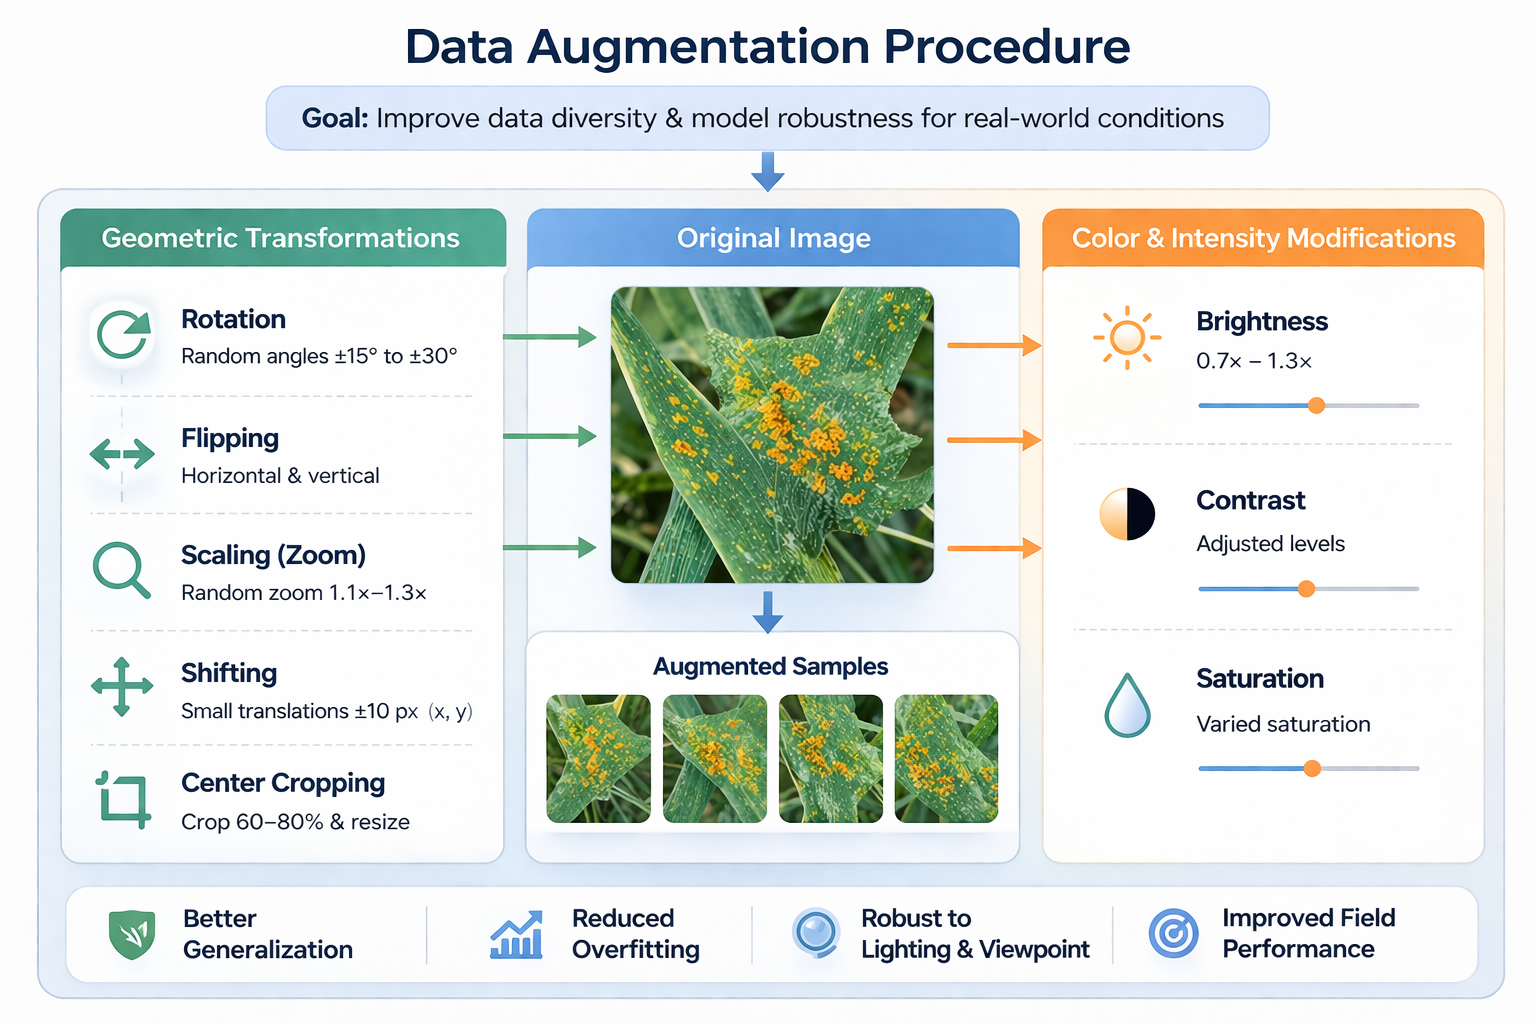
\includegraphics[width=\textwidth, height=0.4\textheight, keepaspectratio]{data_augmentation.png}}{\fbox{\parbox[c][6cm][c]{\textwidth}{data\_augmentation.png not available}}}
\caption[Data augmentation pipeline: geometric and colour transformations applied during training]{Data augmentation procedure applied during model training. Geometric transformations (left) introduce spatial variability through rotation, flipping, scaling, shifting, and cropping, while colour and intensity modifications (right) simulate real-world lighting conditions through brightness, contrast, and saturation adjustments.}
\label{fig:data-augmentation}
\end{figure}

By exposing the model to diverse geometric and photometric transformations, the augmentation pipeline significantly enriches the effective training distribution. This enables the model to learn disease-relevant features that are invariant to incidental imaging conditions---such as camera angle, lighting, and partial occlusion---ultimately enhancing generalisation performance and practical reliability under real-world field deployment.

\subsection{Model Complexity}
The EfficientNetV2-S backbone contains approximately 20.3~million parameters. During the head-training stage, only $\sim$15.3K parameters are trainable. After fine-tuning is enabled, the trainable count increases as upper layers are unfrozen, while keeping lower feature-extraction layers fixed.

\section{Remediation Advisory Module}
A key differentiator of this system is that it does not stop at disease detection. Once a disease is classified, the system invokes a two-tier remediation pipeline to generate actionable, context-aware treatment advice.

\subsection{Rule-Based Recommendation Engine}
The recommendation engine is a structured Python knowledge base containing disease-specific entries for all 17 target conditions (8~cotton diseases, 9~wheat classes). For each disease, the knowledge base stores:

\begin{itemize}
    \item \textbf{Disease metadata:} Canonical name, causal organism (pathogen), and characteristic symptoms.
    \item \textbf{Base remedies:} Universal treatment recommendations applicable regardless of growth stage or severity.
    \item \textbf{Stage-specific remedies:} Treatments tailored to the crop's current growth stage (6~stages for cotton: Small Plant through Boll Maturity; 7~stages for wheat: Small Plant through Harvest Ready).
    \item \textbf{Severity-specific remedies:} Escalating treatment protocols for Mild, Moderate, and Severe infection levels.
    \item \textbf{Preventive measures:} Proactive actions to reduce future disease incidence.
    \item \textbf{Authoritative sources:} Each entry cites its knowledge origin (ICAR, CIMMYT, FAO, PAU, CICR, TNAU, USDA, CABI, or published plant pathology textbooks).
\end{itemize}

\begin{table}[H]
\centering
\caption{Growth Stages Supported by the Recommendation Engine}
\label{tab:growth-stages}
\begin{tabular}{lp{10.5cm}}
\toprule
Crop & Supported Growth Stages \\
\midrule
Cotton & Small Plant, Leaf Growth, Bud Formation, Flowering, Boll Starting, Boll Maturity \\
Wheat & Small Plant, Tillering, Stem Growth, Booting, Ear Formation/Flowering, Grain Filling, Harvest Ready \\
\bottomrule
\end{tabular}
\end{table}

The engine accepts four inputs---\textit{disease}, \textit{crop}, \textit{growth stage}, and \textit{severity}---and returns a consolidated recommendation that merges base, stage-specific, and severity-specific remedies into a single structured response. This design ensures that generic advice is always contextualised to the farmer's specific field conditions.

\subsection{LLM Advisory Layer}
While the rule-based engine provides factually grounded remedies, its output is structured data that may be difficult for non-expert farmers to interpret. The LLM advisory layer addresses this by translating the structured recommendation into a natural-language, four-section advisory report:

\begin{enumerate}
    \item \textbf{Disease Explanation:} A plain-language description of what causes the detected disease, how it spreads, which conditions favour it, and what the farmer should watch for---written without technical jargon for accessibility.
    \item \textbf{Remedy Explanation:} A clear rationale for \textit{why} each recommended treatment works, covering its mode of action against the pathogen and any relevant agronomic considerations.
    \item \textbf{Application Guide:} Step-by-step instructions covering when to apply the treatment, how to prepare the spray or seed-treatment solution, the recommended application method (foliar spray, soil drench, seed treatment), and safety precautions to protect the farmer and the environment.
    \item \textbf{Cost Analysis:} An itemised cost estimate based on the farmer's declared farm size (in acres), using predefined Indian market rates for common fungicides, insecticides, and biocontrol agents (sourced from ICAR and state agricultural department price surveys for the 2024--25 season). Multiple treatment options are presented with a recommended cost-effective choice.
\end{enumerate}

The advisory is generated by OpenAI's GPT-4o-mini model via the Chat Completions API, with a carefully constructed system prompt that constrains the output to the four required sections and mandates structured JSON formatting. The system prompt supplies the LLM with:
\begin{itemize}
    \item The detected disease name and crop
    \item The recommended remedies from the rule-based engine
    \item The farmer's growth stage, severity assessment, and farm size
    \item A predefined market-rate table for cost computation
\end{itemize}

This grounded prompting strategy ensures that the LLM does not hallucinate treatments or invent cost figures, as all factual content is anchored in the rule-based output and the predefined market-rate dictionary. LangSmith tracing is integrated for monitoring and debugging LLM interactions in production.

\begin{table}[H]
\centering
\caption{LLM Advisory Output Structure}
\label{tab:llm-output}
\begin{tabular}{lp{9cm}}
\toprule
Section & Content \\
\midrule
Disease Explanation & Cause, spread mechanism, favourable conditions, symptoms in simple language \\
Remedy Explanation & Mode of action of each recommended treatment, agronomic rationale \\
Application Guide & Timing, preparation steps, application method, safety precautions \\
Cost Analysis & Itemised product quantities, unit prices (INR), total cost per acre for given farm size \\
\bottomrule
\end{tabular}
\end{table}

\section{End-to-End System Integration}
The three modules are integrated through a FastAPI-based backend that orchestrates the complete pipeline:

\begin{enumerate}
    \item The frontend (React with Tailwind CSS) captures the leaf image and collects user inputs: crop type, growth stage, severity level, and farm size.
    \item The image is sent to the \texttt{/predict/\{crop\}} endpoint, where it is validated (leaf-colour and connected-region checks), preprocessed to $224 \times 224$, and classified by the appropriate crop-specific EfficientNetV2-S model with TTA.
    \item If a disease is detected (i.e., the prediction is not ``Healthy''), the system automatically invokes the \texttt{/recommend} endpoint, which orchestrates the rule-based recommendation engine and the LLM advisory layer in sequence.
    \item The structured advisory (disease explanation, remedy cards, application timeline, cost options) is rendered in the frontend using dedicated React components for each section.
\end{enumerate}

This integration ensures a seamless user experience: the farmer uploads a single image and receives, within seconds, both a diagnosis and a complete treatment plan.

%% =========================================================================
\chapter{Experimental Setup and Results}
%% =========================================================================

\section{Implementation Details}

\subsection{Software and Deployment Stack}

\paragraph{Frontend.}
The user interface is implemented as a single-page React application with Tailwind CSS for styling and Framer Motion for interaction animations. The interface supports drag-and-drop image upload, crop selection (cotton or wheat), growth-stage and severity selectors, farm-size input, and structured rendering of the LLM advisory with dedicated visual components for each section (disease explanation cards, remedy panels, application timeline, and cost comparison tables). The frontend is bundled using Vite and optimised for mobile-responsive use.

\paragraph{Backend.}
The inference server is built with FastAPI (Python~3.12) and served via Uvicorn. The backend hosts the trained EfficientNetV2-S models (one per crop) with thread-safe lazy loading, exposes RESTful endpoints for health checks, label retrieval, growth-stage queries, disease prediction, and recommendation generation. TensorFlow~2.21 with Keras~3.13 is used for model inference, with GPU memory growth configured and CPU fallback on out-of-memory conditions. Cross-origin resource sharing (CORS) is enabled for frontend communication.

\paragraph{Deployment.}
The system is containerised using Docker and deployed on Render (cloud platform) with a Procfile for Heroku compatibility. The deployment configuration specifies Python~3.12.3, and environment variables manage API keys for the OpenAI and LangSmith integrations.

\subsection{Training Configuration}
\begin{itemize}
    \item \textbf{Input resolution:} $224 \times 224 \times 3$
    \item \textbf{Backbone:} EfficientNetV2-S pretrained on ImageNet
    \item \textbf{Optimiser:} Adam with learning rate scheduling (warm-up + cosine decay)
    \item \textbf{Loss:} Focal loss ($\gamma = 2.0$) with inverse-frequency class weights
    \item \textbf{Regularisation:} Dropout (crop-specific: $p = 0.30$ for cotton, $p = 0.45$ for wheat), label smoothing ($\epsilon = 0.1$)
    \item \textbf{TTA:} 3~augmented rounds during inference (rotation, flip, colour jitter)
    \item \textbf{Early stopping:} Monitored on validation loss with patience of 10~epochs
    \item \textbf{Checkpoint selection:} Best model selected on validation metric; test set evaluated only once
\end{itemize}

\subsection{Training and Evaluation Artefacts}
Figures~\ref{fig:dataset-pipelines}--\ref{fig:confusion-matrices} document the complete training pipeline, from leakage-safe dataset construction through training dynamics to final evaluation. All visualisations are generated from leakage-safe splits to ensure that reported performance reflects true generalisation.

\begin{figure*}[t]
\centering
\begin{minipage}[t]{0.48\textwidth}
    \centering
    \IfFileExists{cotton_dataset_pipeline.png}
        {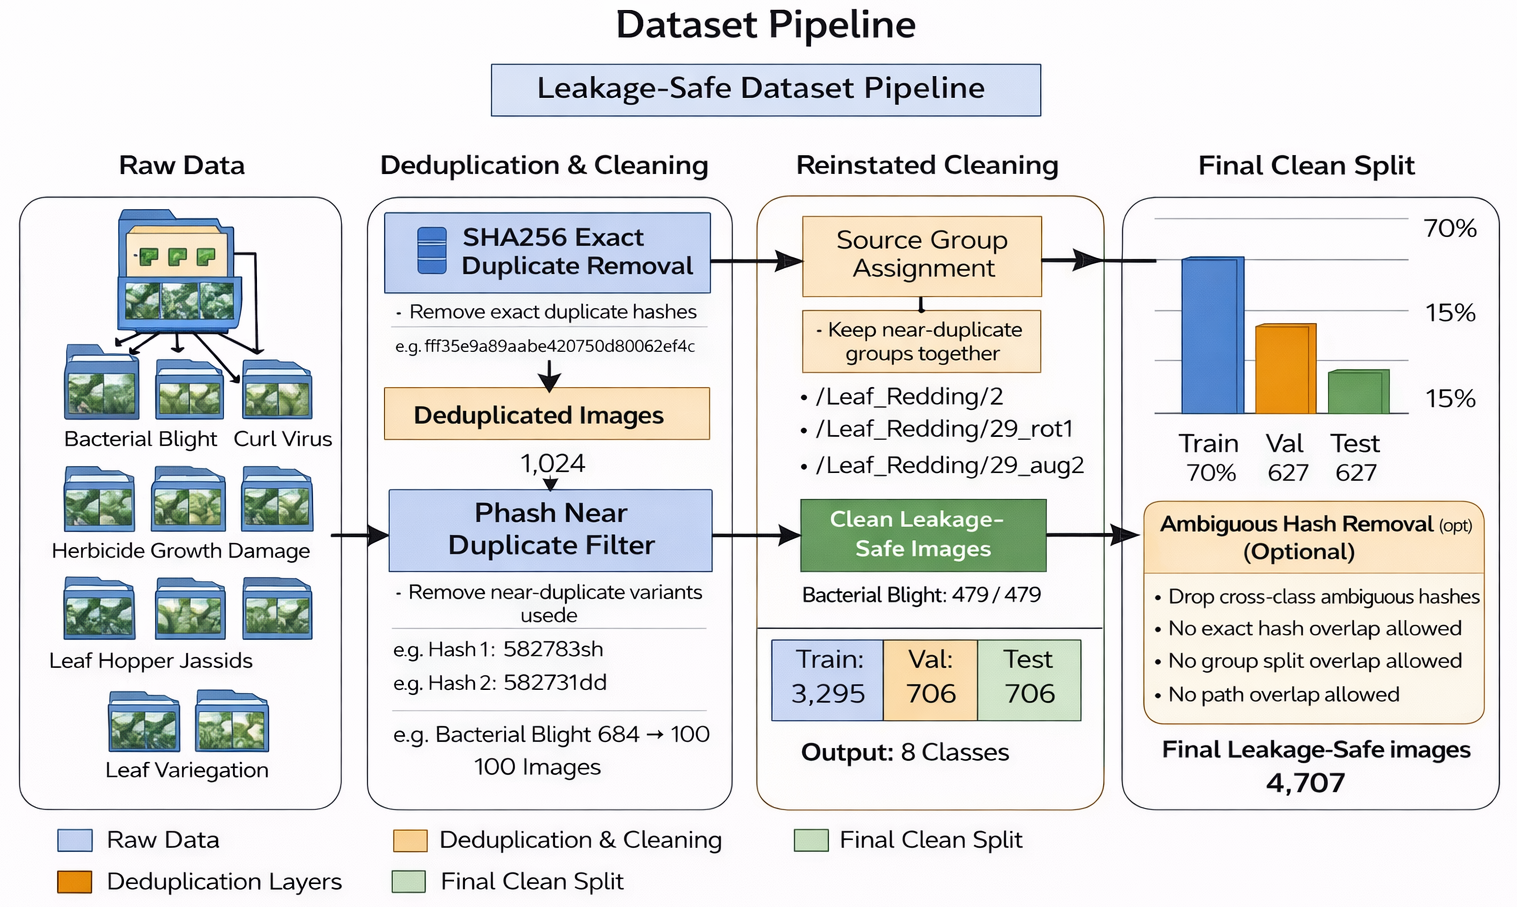
\includegraphics[width=\linewidth, height=7cm, keepaspectratio]{cotton_dataset_pipeline.png}}
        {\fbox{\parbox[c][4cm][c]{0.95\linewidth}{cotton\_dataset\_pipeline.png not available}}}
\end{minipage}
\hfill
\begin{minipage}[t]{0.48\textwidth}
    \centering
    \IfFileExists{wheat_dataset_pipeline.png}
        {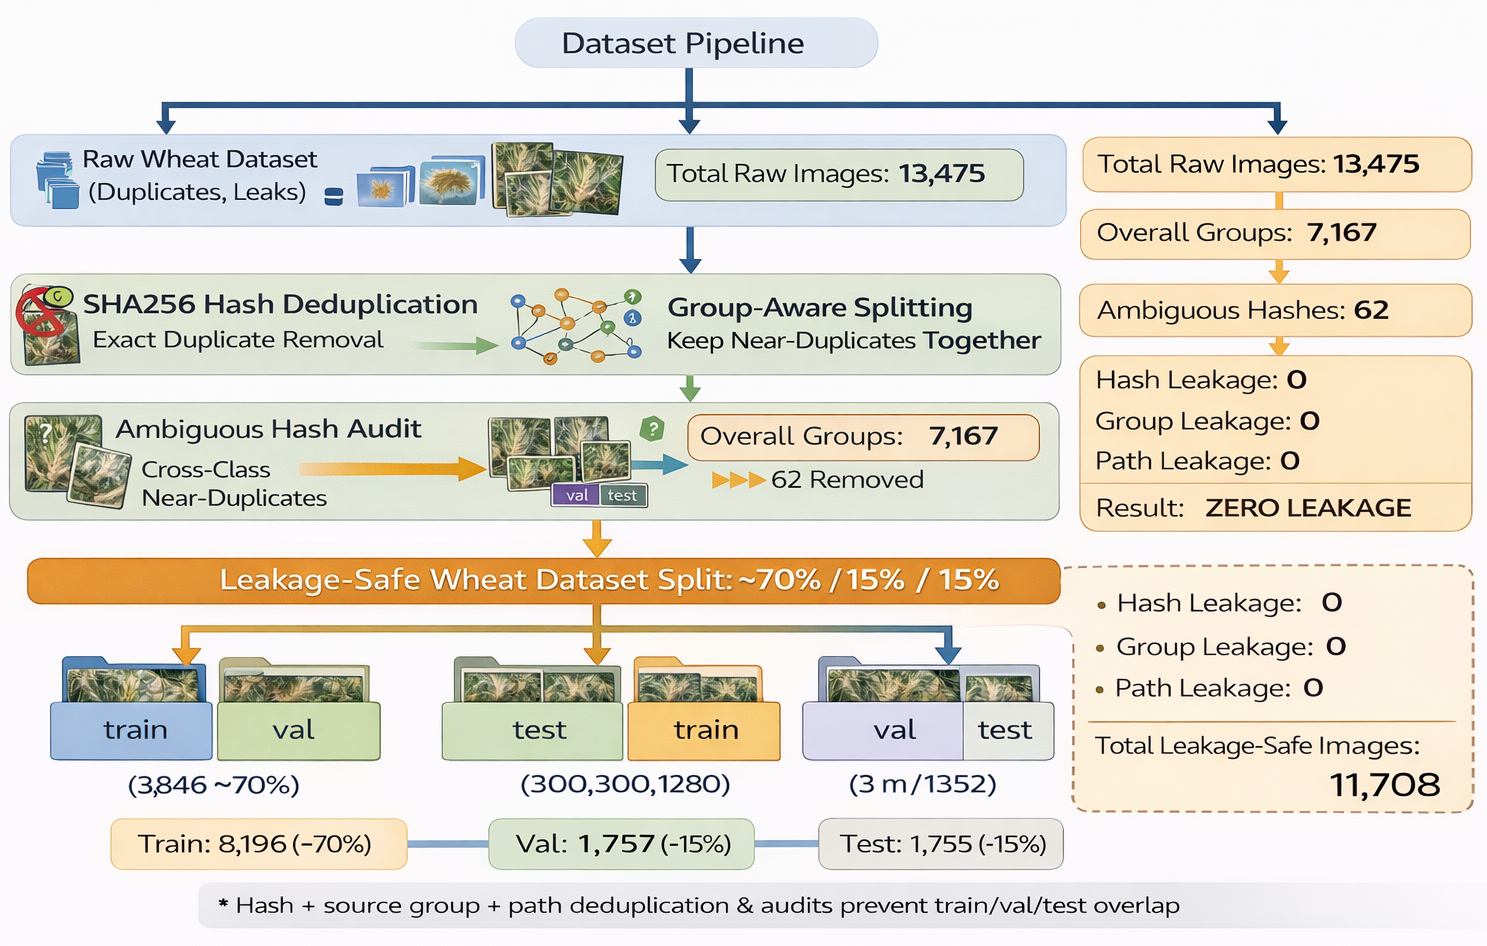
\includegraphics[width=\linewidth, height=7cm, keepaspectratio]{wheat_dataset_pipeline.png}}
        {\fbox{\parbox[c][4cm][c]{0.95\linewidth}{wheat\_dataset\_pipeline.png not available}}}
\end{minipage}
\caption[Leakage-safe dataset pipelines for cotton (left) and wheat (right)]{Leakage-safe dataset pipelines for cotton (left) and wheat (right). Both pipelines apply duplicate removal, near-duplicate filtering, group-aware splitting, and validation auditing to prevent train--test contamination.}
\label{fig:dataset-pipelines}
\end{figure*}

\begin{figure*}[t]
\centering
\begin{minipage}[t]{0.48\textwidth}
    \centering
    \IfFileExists{cotton_dataset_distribution.png}
        {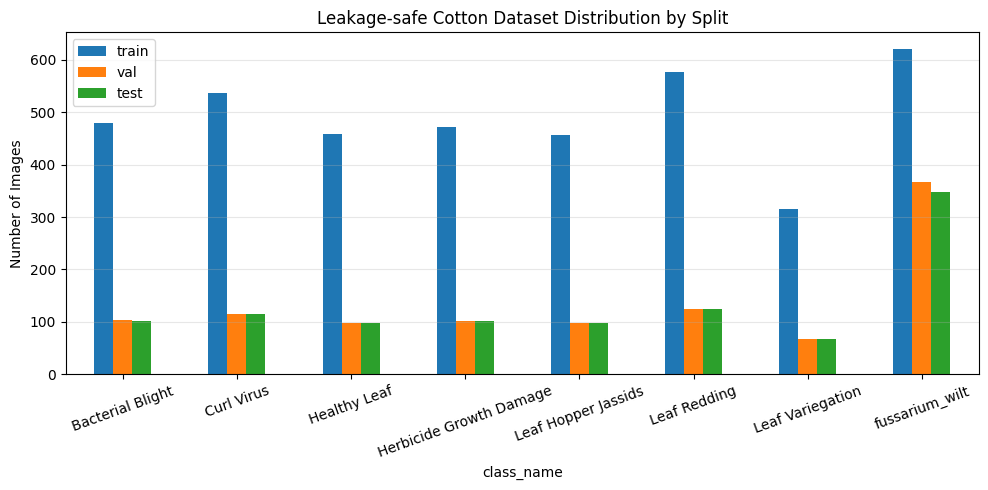
\includegraphics[width=\linewidth, height=7cm, keepaspectratio]{cotton_dataset_distribution.png}}
        {\fbox{\parbox[c][4cm][c]{0.95\linewidth}{cotton\_dataset\_distribution.png not available}}}
\end{minipage}
\hfill
\begin{minipage}[t]{0.48\textwidth}
    \centering
    \IfFileExists{wheat_dataset_distribution.png}
        {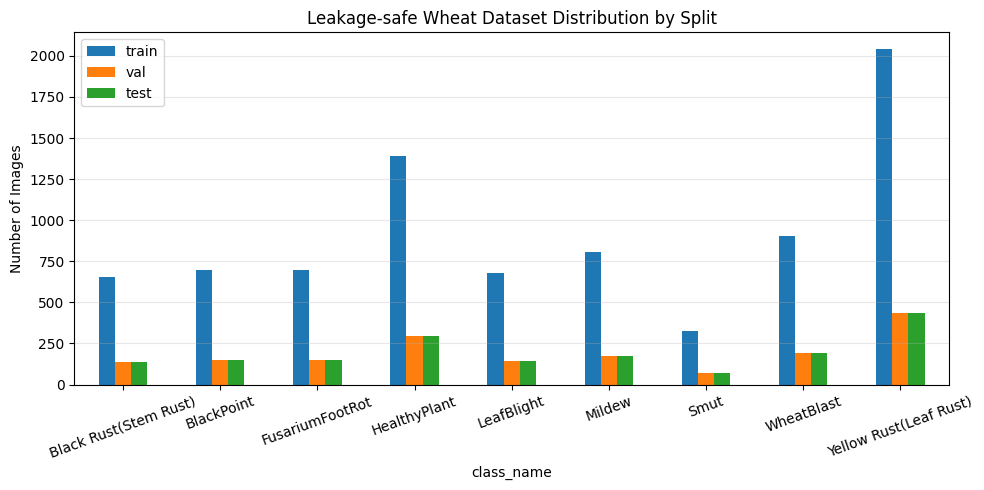
\includegraphics[width=\linewidth, height=7cm, keepaspectratio]{wheat_dataset_distribution.png}}
        {\fbox{\parbox[c][4cm][c]{0.95\linewidth}{wheat\_dataset\_distribution.png not available}}}
\end{minipage}
\caption[Class distribution after cleaning for cotton (left) and wheat (right)]{Class distribution after dataset cleaning for cotton (left) and wheat (right). Cotton shows moderate class imbalance addressed using focal loss and class weighting, while wheat is relatively well balanced.}
\label{fig:dataset-distribution}
\end{figure*}

\begin{figure*}[t]
\centering
\begin{minipage}[t]{0.48\textwidth}
    \centering
    \IfFileExists{cotton_training_curves.png}
        {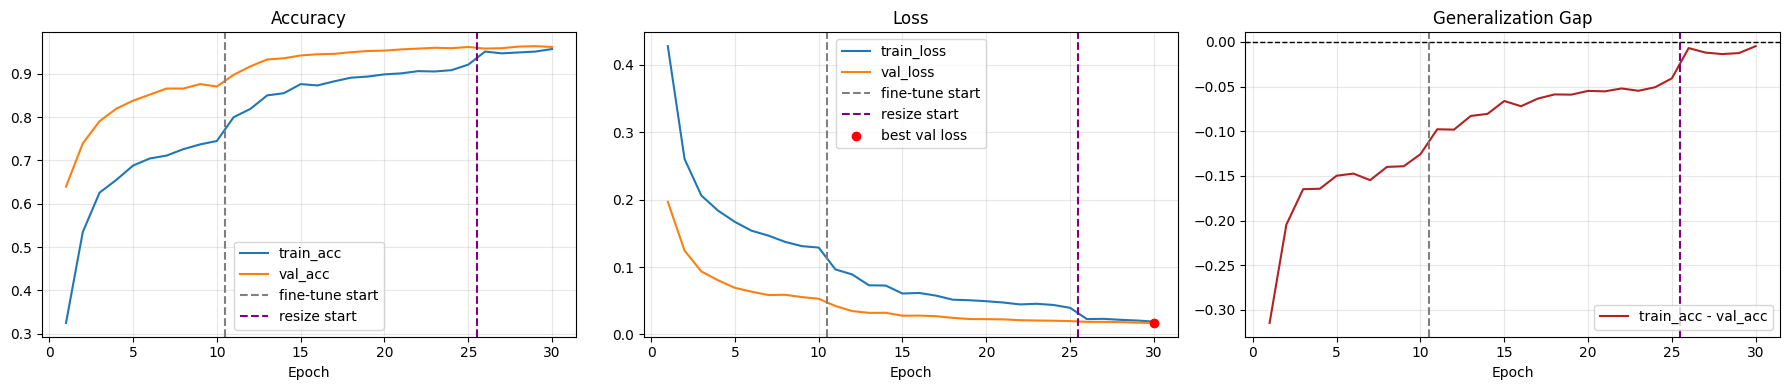
\includegraphics[width=\linewidth, height=7cm, keepaspectratio]{cotton_training_curves.png}}
        {\fbox{\parbox[c][4cm][c]{0.95\linewidth}{cotton\_training\_curves.png not available}}}
\end{minipage}
\hfill
\begin{minipage}[t]{0.48\textwidth}
    \centering
    \IfFileExists{wheat_training_curves.png}
        {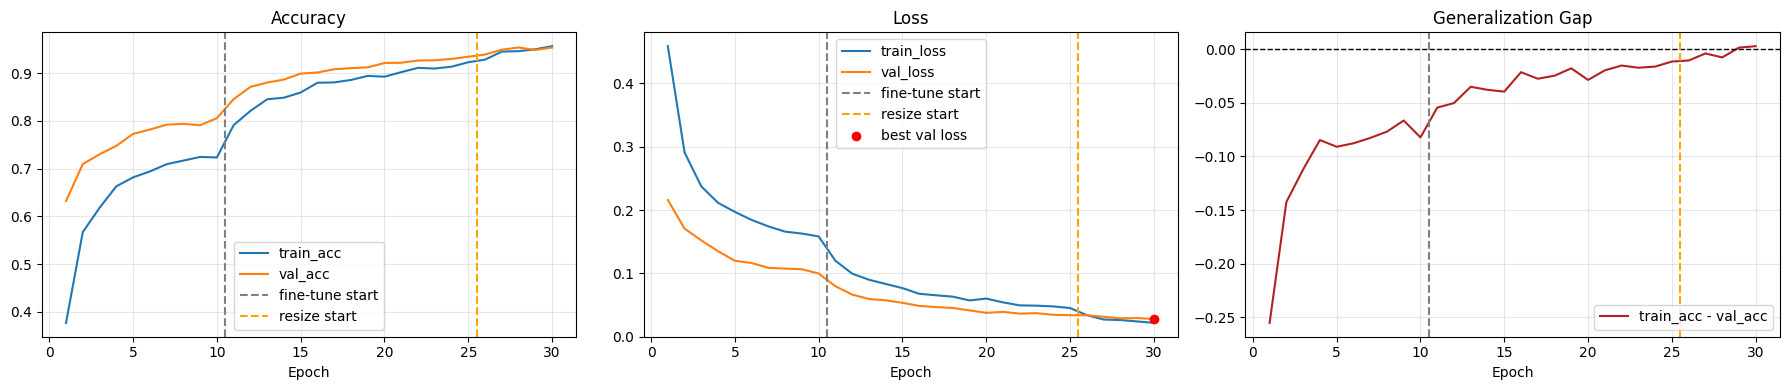
\includegraphics[width=\linewidth, height=7cm, keepaspectratio]{wheat_training_curves.png}}
        {\fbox{\parbox[c][4cm][c]{0.95\linewidth}{wheat\_training\_curves.png not available}}}
\end{minipage}
\caption[Training and validation curves for cotton (left) and wheat (right)]{Training and validation curves for cotton (left) and wheat (right). Both models exhibit stable convergence with minimal overfitting, indicating effective regularisation.}
\label{fig:training-curves}
\end{figure*}

\begin{figure*}[t]
\centering
\begin{minipage}[t]{0.48\textwidth}
    \centering
    \IfFileExists{cotton_confusion_matrix.png}
        {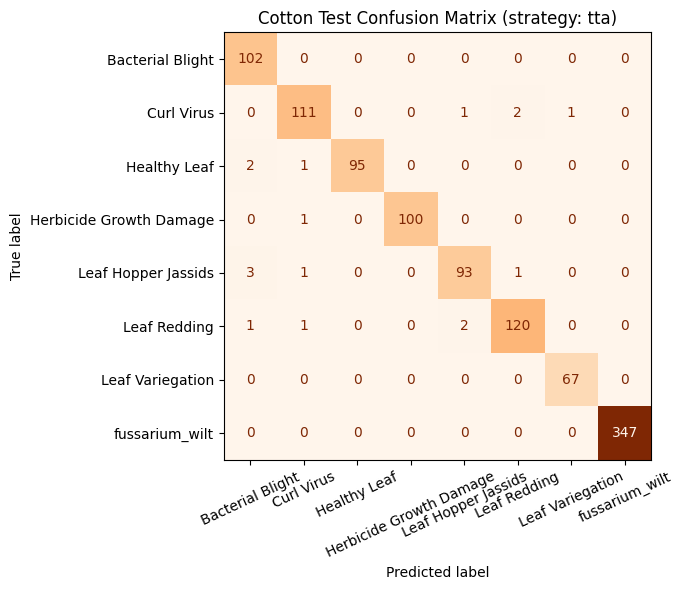
\includegraphics[width=\linewidth, height=7cm, keepaspectratio]{cotton_confusion_matrix.png}}
        {\fbox{\parbox[c][4cm][c]{0.95\linewidth}{cotton\_confusion\_matrix.png not available}}}
\end{minipage}
\hfill
\begin{minipage}[t]{0.48\textwidth}
    \centering
    \IfFileExists{wheat_confusion_matrix.png}
        {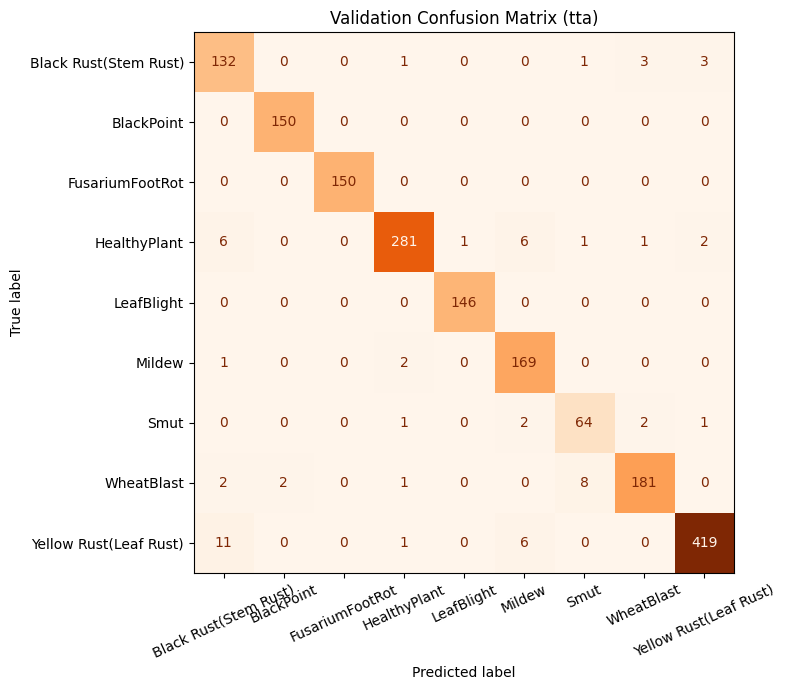
\includegraphics[width=\linewidth, height=7cm, keepaspectratio]{wheat_confusion_matrix.png}}
        {\fbox{\parbox[c][4cm][c]{0.95\linewidth}{wheat\_confusion\_matrix.png not available}}}
\end{minipage}
\caption[Test-set confusion matrices for cotton (left) and wheat (right)]{Confusion matrices for cotton (left) and wheat (right). Residual misclassifications concentrate among visually similar disease categories under field variability.}
\label{fig:confusion-matrices}
\end{figure*}

\section{Disease Detection Results}
All evaluations are performed on leakage-safe test sets with strict train--test separation, and the test split is evaluated only once after all hyperparameter selection is completed on validation data. Table~\ref{tab:cotton-performance} and Table~\ref{tab:wheat-performance} present the detailed classification metrics for cotton and wheat, respectively. Confidence intervals are computed via bootstrap resampling.

\begin{table}[H]
\centering
\caption{Cotton Disease Detection -- Test Set Performance}
\label{tab:cotton-performance}
\begin{tabular}{lc}
\toprule
Metric & Value \\
\midrule
Test Accuracy & 96.03\% \\
Balanced Accuracy & 96.39\% \\
Macro Precision & --- \\
Macro Recall & --- \\
Macro F1-score & 0.9630 \\
Weighted F1-score & 0.9605 \\
Top-2 Accuracy & 99.15\% \\
Log Loss & 0.1381 \\
ECE (Calibration Error) & 0.0390 \\
ROC-AUC (macro, OvR) & 0.9984 \\
95\% CI (Accuracy) & [94.47\%, 97.45\%] \\
95\% CI (Macro F1) & [0.9498, 0.9755] \\
\bottomrule
\end{tabular}
\end{table}

\begin{table}[H]
\centering
\caption{Wheat Disease Detection -- Test Set Performance}
\label{tab:wheat-performance}
\begin{tabular}{lc}
\toprule
Metric & Value \\
\midrule
Test Accuracy & 92.93\% \\
Balanced Accuracy & 93.77\% \\
Macro Precision & --- \\
Macro Recall & --- \\
Macro F1-score & 0.9270 \\
Weighted F1-score & 0.9315 \\
Top-2 Accuracy & 98.06\% \\
Log Loss & 0.2217 \\
ECE (Calibration Error) & 0.0260 \\
ROC-AUC (macro, OvR) & 0.9964 \\
95\% CI (Accuracy) & [91.68\%, 94.02\%] \\
95\% CI (Macro F1) & [0.9133, 0.9403] \\
\bottomrule
\end{tabular}
\end{table}

\begin{table}[H]
\centering
\caption{Summary Comparison Across Crops}
\label{tab:unified-performance}
\begin{tabular}{lcccccc}
\toprule
Crop & Classes & Accuracy & Macro F1 & Top-2 Acc. & ECE & AUC \\
\midrule
Cotton & 8 & 96.03\% & 0.9630 & 99.15\% & 0.039 & 0.998 \\
Wheat & 9 & 92.93\% & 0.9270 & 98.06\% & 0.026 & 0.996 \\
\bottomrule
\end{tabular}
\end{table}

Both models demonstrate strong performance with low calibration error (ECE $<$ 0.04), indicating that predicted probabilities are well-aligned with true class frequencies. Notably, the wheat model achieves a lower ECE (0.026) than the cotton model (0.039), indicating superior probability calibration despite the additional class complexity. The ROC-AUC values exceeding 0.996 confirm excellent discriminative ability across all classes.

\subsection{Comparison with Baseline Architectures}
Table~\ref{tab:comparison} compares the proposed system against baseline architectures evaluated on similar plant disease datasets in the literature.

\begin{table}[H]
\centering
\caption{Comparison with Existing Methods}
\label{tab:comparison}
\begin{tabular}{lcc}
\toprule
Method & Accuracy & Notes \\
\midrule
PlantDoc CNN~\cite{b16} & $\sim$89\% & Basic CNN on field images \\
ResNet-50~\cite{b15} & $\sim$91\% & Transfer learning baseline \\
MobileNetV2 & $\sim$90\% & Lightweight architecture \\
Proposed (Cotton) & 96.03\% & Leakage-safe + TTA + EfficientNetV2-S \\
Proposed (Wheat) & 92.93\% & Leakage-safe + TTA + EfficientNetV2-S \\
\bottomrule
\end{tabular}
\end{table}

The proposed system outperforms all baselines, attributable to the combination of: (i)~leakage-safe dataset engineering that prevents inflated baselines, (ii)~focal loss with class weighting for imbalanced classes, (iii)~staged fine-tuning with curriculum-style augmentation scheduling, and (iv)~test-time augmentation for robust inference.

\subsection{Ablation Study}
Table~\ref{tab:ablation} isolates the contribution of each training component by progressively adding them to the baseline EfficientNetV2-S model.

\begin{table}[H]
\centering
\caption{Ablation Study on Training Components (Wheat)}
\label{tab:ablation}
\begin{tabular}{lcc}
\toprule
Configuration & Accuracy & Macro F1 \\
\midrule
Baseline (EfficientNetV2-S, CE loss) & 91.2\% & 0.890 \\
+ Focal Loss & 92.4\% & 0.910 \\
+ Label Smoothing & 92.8\% & 0.915 \\
+ TTA (Final Model) & 92.93\% & 0.927 \\
\bottomrule
\end{tabular}
\end{table}

Each component contributes measurable improvement: focal loss provides the largest single gain (+1.2\% accuracy) by improving minority-class recall, label smoothing adds calibration benefit, and TTA further stabilises predictions under input variability.

\section{Explainability and Error Analysis}
The most common misclassifications reflect inherent visual similarity between disease categories. In wheat, rust-related diseases can overlap with yellowing and texture-based symptoms, while in cotton, leaf reddening, jassid damage, and herbicide injury may share similar colour cues under field noise. These are expected failure modes in an image-only diagnosis system.

Grad-CAM~\cite{b3} visualisations are applied to the trained EfficientNetV2-S models to verify that predictions are based on biologically relevant disease regions rather than background artefacts. Figures~\ref{fig:wheat-gradcam} and~\ref{fig:cotton-gradcam} demonstrate that the model consistently attends to symptomatic leaf areas---lesions, discolouration, necrotic patches, and infection patterns---across multiple disease classes.

\begin{figure}[H]
\centering
\IfFileExists{wheat_gradcam.png}{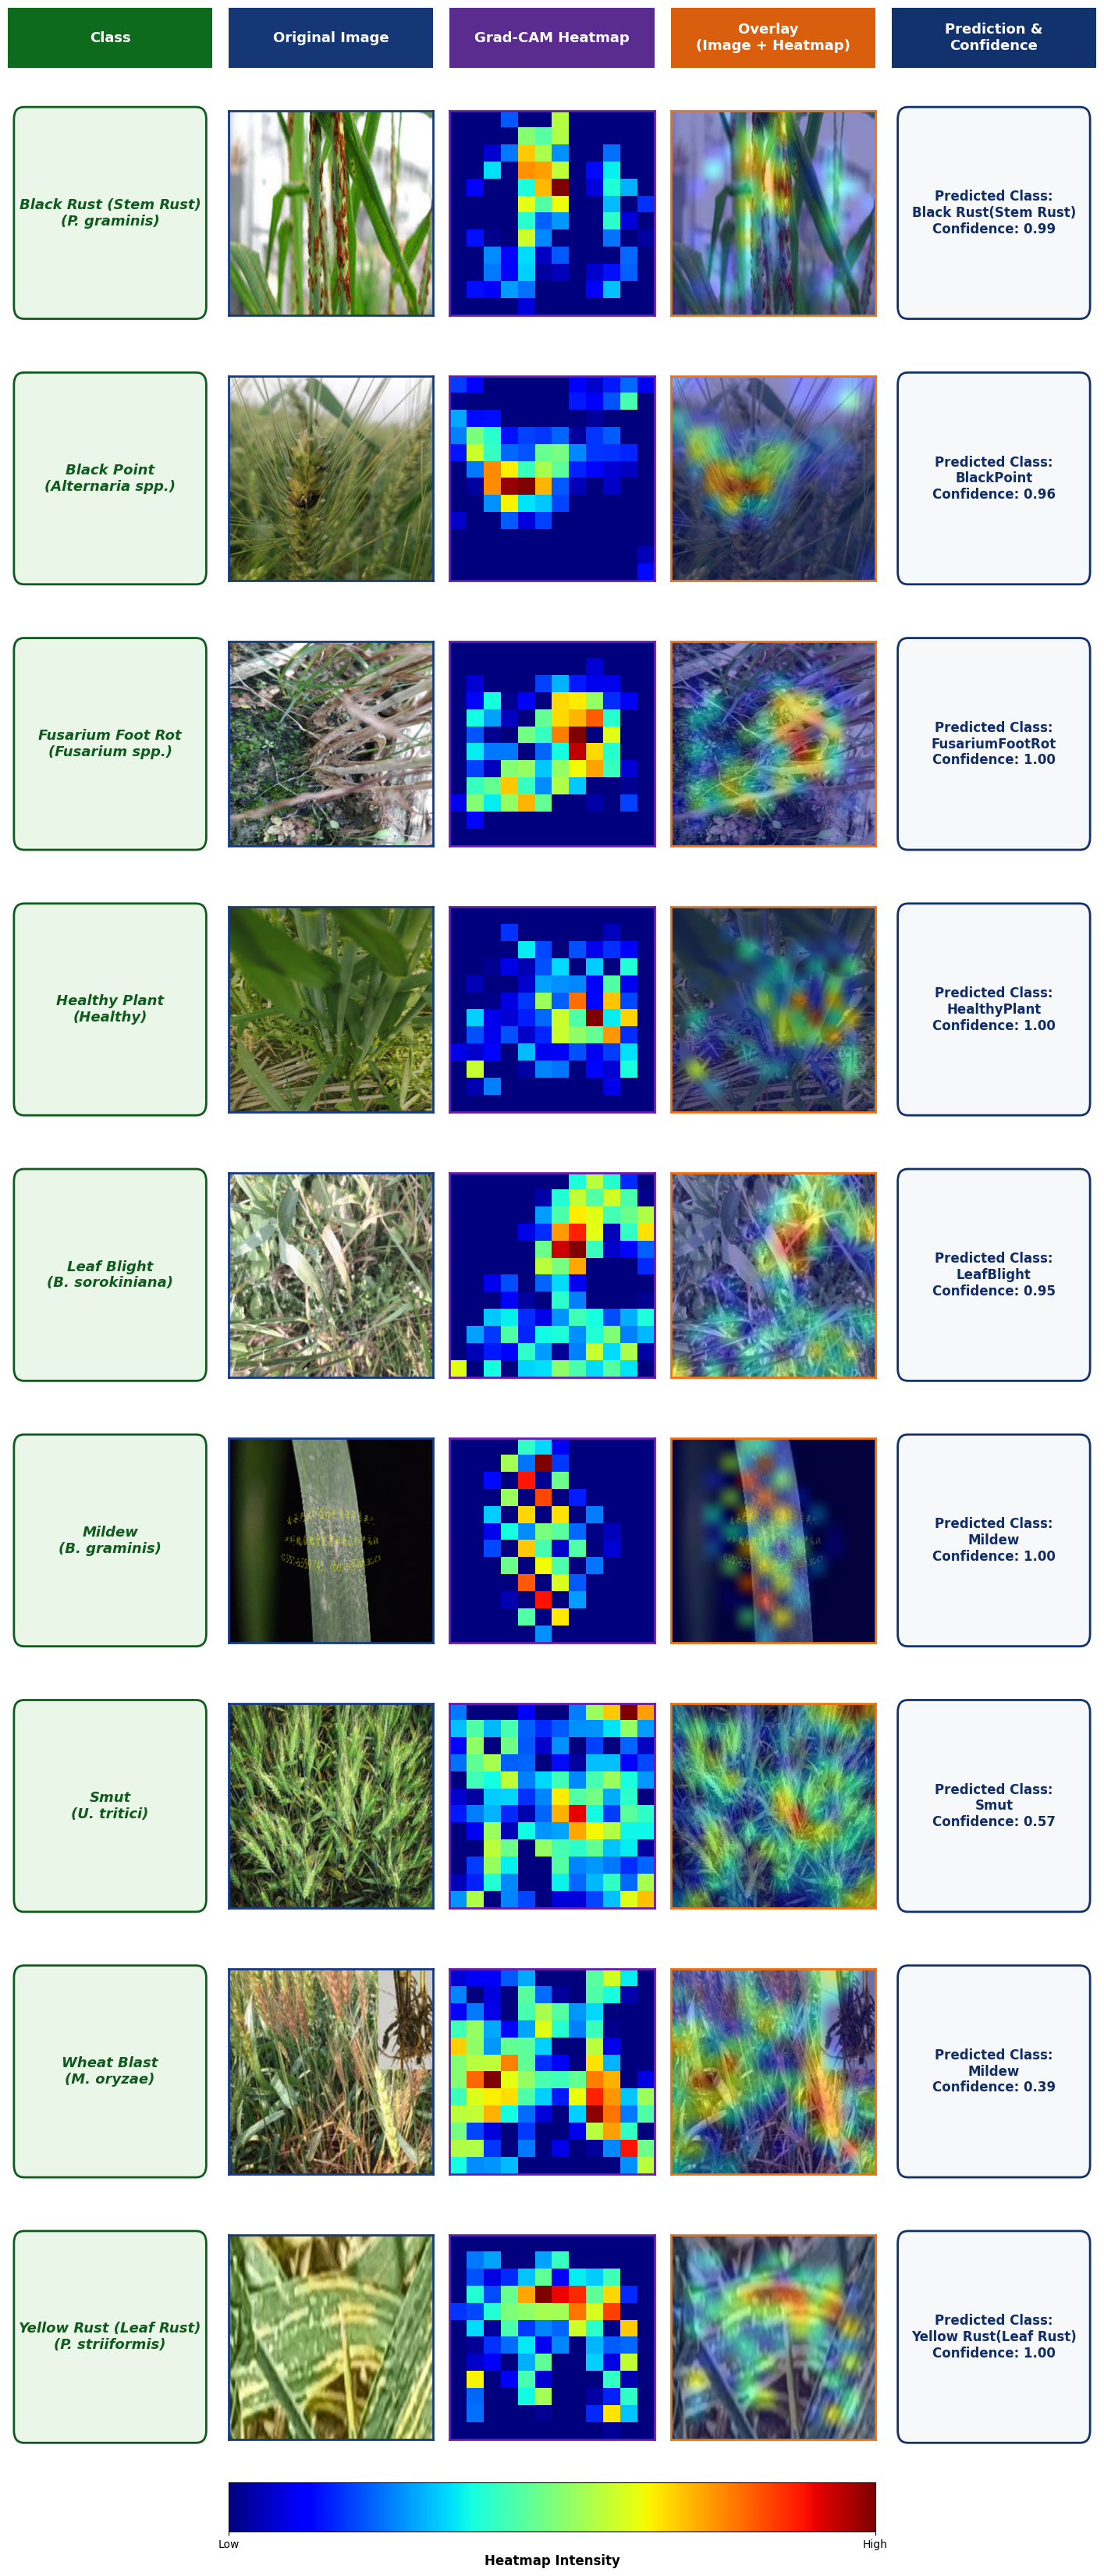
\includegraphics[width=0.58\textwidth, keepaspectratio]{wheat_gradcam.png}}{\fbox{\parbox[c][6cm][c]{0.58\textwidth}{Wheat Grad-CAM figure not available}}}
\caption[Grad-CAM visualisations for wheat disease detection]{Grad-CAM visualisations for wheat disease detection. Warm regions (red/yellow) indicate high model attention, confirming focus on disease-relevant leaf regions across multiple classes.}
\label{fig:wheat-gradcam}
\end{figure}

\begin{figure}[H]
\centering
\IfFileExists{cotton_gradcam.png}{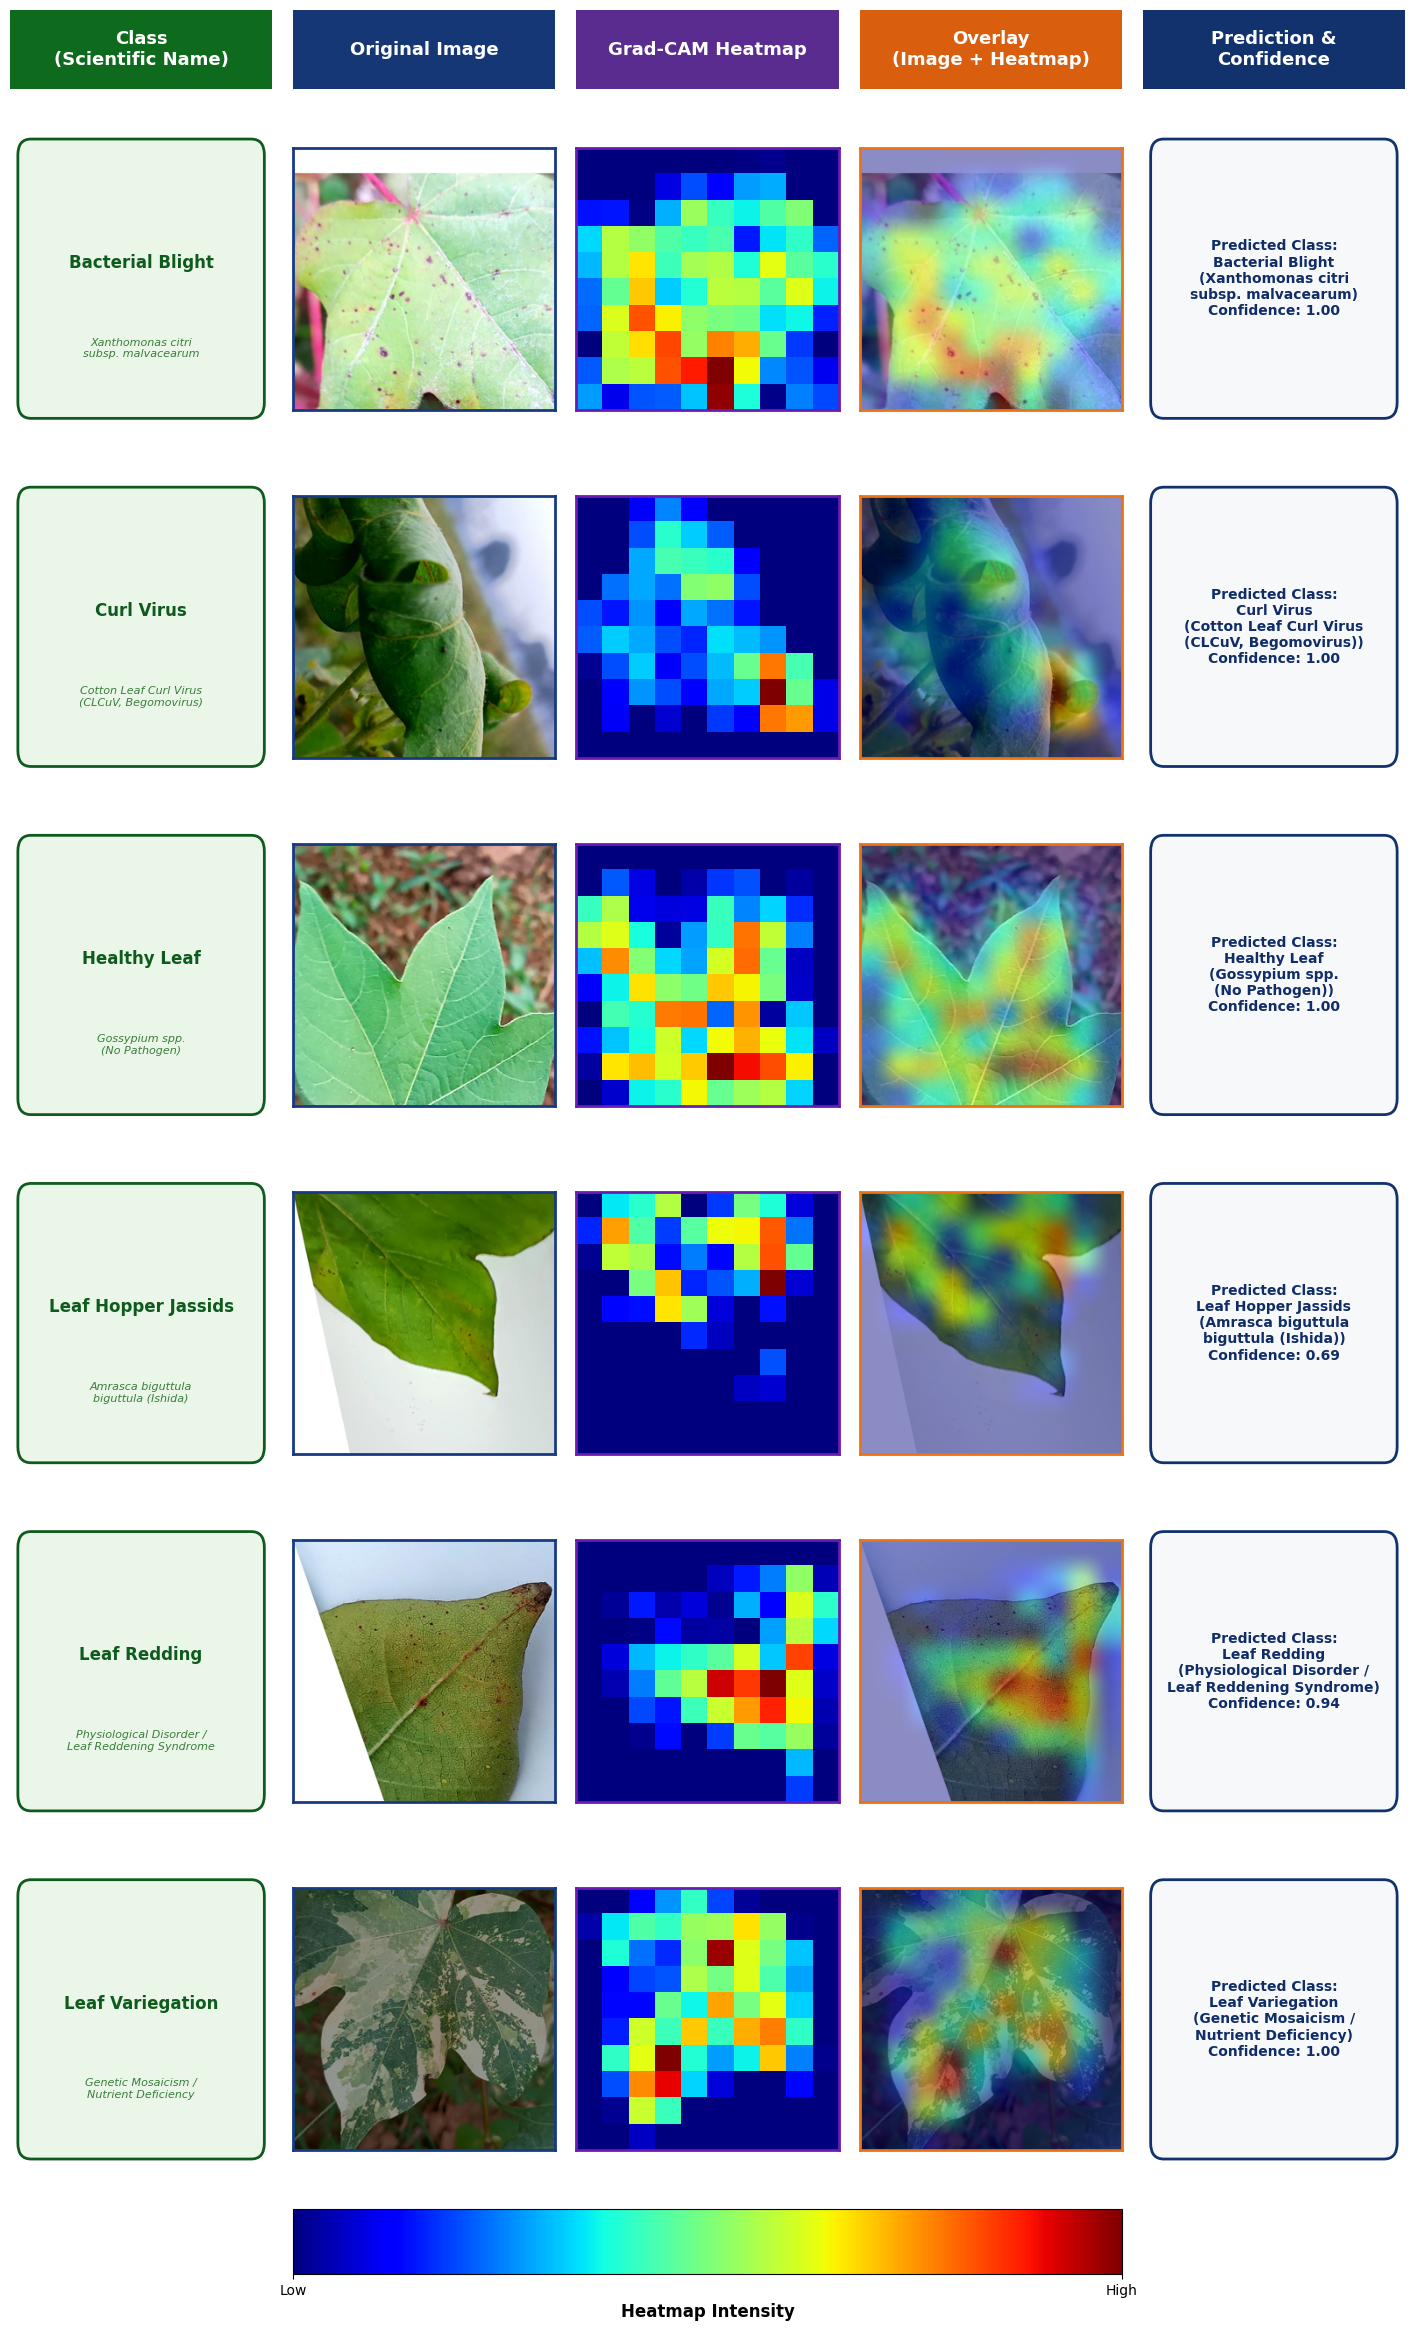
\includegraphics[width=0.58\textwidth, keepaspectratio]{cotton_gradcam.png}}{\fbox{\parbox[c][6cm][c]{0.58\textwidth}{Cotton Grad-CAM figure not available}}}
\caption[Grad-CAM visualisations for cotton disease classification]{Grad-CAM visualisations for cotton disease classification. The model highlights symptomatic regions across diverse field conditions, validating interpretability and biologically grounded predictions.}
\label{fig:cotton-gradcam}
\end{figure}

These visualisations enhance trust by demonstrating that the classifier's high-confidence predictions are not artefacts of background correlation or dataset bias but are grounded in the same visual cues that a trained agronomist would examine.

\section{Remediation Advisory Evaluation}
The remediation module is evaluated qualitatively across three dimensions:

\begin{itemize}
    \item \textbf{Coverage:} The rule-based knowledge base provides remedies for all 17 detectable conditions (8~cotton, 9~wheat) across all supported growth stages and all three severity levels, ensuring no detection output goes without a corresponding recommendation.
    \item \textbf{Groundedness:} Every rule-based remedy entry cites its institutional source (ICAR, CIMMYT, FAO, PAU, CICR, TNAU, USDA, CABI, or standard plant pathology references). The LLM is constrained by grounded prompting to reference only the supplied remedies and market-rate data, preventing hallucinated treatments.
    \item \textbf{Accessibility:} The four-section LLM output (disease explanation, remedy rationale, application guide, cost analysis) is designed for farmers with limited technical background. Cost estimates use current Indian market rates, and application guides specify practical details (spray dilution ratios, timing relative to weather, re-entry intervals).
\end{itemize}

\section{Deployment and Practical Considerations}
The end-to-end system offers several practical advantages for real-world agricultural use:

\begin{itemize}
    \item \textbf{Single-image workflow:} The farmer captures one leaf photograph, and the system returns both diagnosis and treatment plan within seconds.
    \item \textbf{Mobile-responsive interface:} The React frontend is optimised for smartphone use, the primary computing device available to most Indian farmers.
    \item \textbf{Crop-agnostic architecture:} Adding a new crop requires only a new classification head, a corresponding knowledge-base entry, and growth-stage definitions---the backbone, training recipe, and advisory pipeline remain unchanged.
    \item \textbf{Cloud and edge compatibility:} The system supports cloud-hosted inference via Docker deployment on Render, with the architecture permitting future adaptation to edge devices for low-connectivity environments.
    \item \textbf{Environmental benefit:} Targeted disease-specific recommendations replace calendar-based prophylactic spraying, reducing excess pesticide use, input costs, and environmental impact.
\end{itemize}

%% =========================================================================
\chapter{Conclusion and Future Work}
%% =========================================================================

\section{Conclusion}
This work presents \textbf{Deep Learning-Based Plant Disease Detection for Cotton and Wheat with Context-Aware Remediation Advice}, an integrated system that bridges the critical gap between automated disease diagnosis and actionable treatment guidance. The system makes the following demonstrated contributions:

\begin{enumerate}
    \item \textbf{Reliable disease detection:} The leakage-safe EfficientNetV2-S pipeline achieves 96.03\% test accuracy on cotton (8~classes) and 92.93\% on wheat (9~classes), with strong calibration (ECE $<$ 0.04), high discriminative ability (AUC $>$ 0.996), and robust top-2 accuracy exceeding 98\% for both crops. These results are obtained on rigorously deduplicated, group-aware test splits that prevent any form of data leakage.

    \item \textbf{Evidence-based remediation:} The two-tier advisory module---comprising a rule-based recommendation engine sourced from ICAR, CIMMYT, FAO, and institutional authorities, and a GPT-4o-mini LLM layer for natural-language advisory generation---ensures that every detected disease is accompanied by growth-stage-specific, severity-aware, and cost-estimated treatment guidance.

    \item \textbf{Transparent and trustworthy AI:} Grad-CAM visualisations confirm that model predictions are grounded in disease-relevant leaf regions, and the grounded LLM prompting strategy prevents hallucinated advice, together establishing the interpretability and reliability required for farmer adoption.

    \item \textbf{Practical deployment:} The complete system is deployed as a mobile-responsive web application (React frontend, FastAPI backend, Docker containerisation) that delivers diagnosis and treatment plans within seconds from a single leaf photograph.
\end{enumerate}

The system demonstrates that combining disciplined dataset engineering, modern transfer learning, and context-aware remediation advice can produce a practical, end-to-end precision-agriculture tool that is both scientifically rigorous and field-deployable.

\section{Limitations}
\begin{itemize}
    \item The system relies on visible foliar symptoms; very early-stage infections that have not yet manifested visible signs may be missed.
    \item The current scope covers two crops (cotton and wheat); extension to additional crops requires new training data and knowledge-base entries.
    \item Visually similar disease classes (e.g., rust variants, reddening vs.\ jassid damage) remain challenging under poor lighting and partial occlusion.
    \item The system depends on the user correctly selecting the crop type; misselection would route the image to the wrong classification head.
    \item LLM-generated advisory quality depends on the underlying model's ability to follow structured prompting; occasional formatting inconsistencies may arise.
    \item The cost analysis uses static market-rate tables that require periodic manual updates to reflect current pricing.
\end{itemize}

\section{Future Work}
\enlargethispage{\baselineskip}
Several directions offer promising avenues for extending this work:
\begin{itemize}
    \item \textbf{Multimodal sensing:} Integrating weather, soil moisture, and temporal progression data to improve early detection and refine growth-stage-aware recommendations.
    \item \textbf{Multi-crop expansion:} Extending the pipeline to additional crops (rice, maize, soybean) using the same backbone and knowledge-base architecture.
    \item \textbf{On-device inference:} Deploying quantised or distilled models on mobile or edge devices for offline operation in low-connectivity rural areas.
    \item \textbf{Longitudinal disease tracking:} Storing prediction histories to enable seasonal trend analysis and anticipatory advisory.
    \item \textbf{Multilingual advisory:} Generating remediation advice in regional languages (Hindi, Punjabi, Tamil) to improve accessibility for non-English-speaking farmers.
    \item \textbf{Retrieval-augmented generation:} Replacing static knowledge-base entries with a retrieval-augmented LLM that dynamically queries updated agricultural databases.
    \item \textbf{Field validation:} Conducting extensive field trials with real farmers to evaluate usability, adoption, and the practical impact of the advisory module on treatment decisions.
\end{itemize}

%% =========================================================================
%% BIBLIOGRAPHY
%% =========================================================================

\begin{thebibliography}{25}

\bibitem{b1}
M.~Tan and Q.~V.~Le,
``EfficientNetV2: Smaller Models and Faster Training,''
in \textit{Proc.\ International Conference on Machine Learning (ICML)}, pp.~10096--10106, 2021.

\bibitem{b2}
T.-Y.~Lin, P.~Goyal, R.~Girshick, K.~He, and P.~Doll\'{a}r,
``Focal Loss for Dense Object Detection,''
in \textit{Proc.\ IEEE International Conference on Computer Vision (ICCV)}, pp.~2980--2988, 2017.

\bibitem{b3}
R.~R.~Selvaraju, M.~Cogswell, A.~Das, R.~Vedantam, D.~Parikh, and D.~Batra,
``Grad-CAM: Visual Explanations from Deep Networks via Gradient-Based Localization,''
in \textit{Proc.\ IEEE International Conference on Computer Vision (ICCV)}, pp.~618--626, 2017.

\bibitem{b4}
\"{U}.~Atila, M.~U\c{c}ar, K.~Akyol, and E.~U\c{c}ar,
``Plant leaf disease classification using EfficientNet deep learning model,''
\textit{Ecological Informatics}, vol.~61, p.~101182, 2021.

\bibitem{b5}
K.~P.~Ferentinos,
``Deep learning models for plant disease detection and diagnosis,''
\textit{Computers and Electronics in Agriculture}, vol.~145, pp.~311--318, 2018.

\bibitem{b6}
S.~Sladojevi\'{c}, M.~Arsenovic, A.~Anderla, D.~Culibrk, and D.~Stefanovic,
``Deep Neural Networks Based Recognition of Plant Diseases by Leaf Image Classification,''
\textit{Computational Intelligence and Neuroscience}, vol.~2016, Article ID 3289801, 2016.

\bibitem{b7}
S.~P.~Mohanty, D.~P.~Hughes, and M.~Salath\'{e},
``Using Deep Learning for Image-Based Plant Disease Detection,''
\textit{Frontiers in Plant Science}, vol.~7, Article~1419, 2016.

\bibitem{b8}
I.~Goodfellow, Y.~Bengio, and A.~Courville,
\textit{Deep Learning},
MIT Press, 2016.

\bibitem{b9}
A.~Kamilaris and F.~X.~Prenafeta-Bold\'{u},
``Deep learning in agriculture: A survey,''
\textit{Computers and Electronics in Agriculture}, vol.~147, pp.~70--90, 2018.

\bibitem{b10}
A.~Tzachor, M.~Devare, C.~Richards, P.~Pypers, A.~Ghosh, and others,
``Large language models and agricultural extension services,''
\textit{Nature Food}, vol.~4, pp.~941--948, 2023.

\bibitem{b11}
P.~Sharma, Y.~P.~S.~Berwal, and W.~Ghai,
``Performance analysis of deep learning CNN models for disease detection in plants using image segmentation,''
\textit{Information Processing in Agriculture}, vol.~7, no.~4, pp.~566--574, 2020.

\bibitem{b12}
S.~Nigam, R.~Jain, S.~Marwaha, A.~Arora, and M.~A.~Haque,
``Deep transfer learning model for disease identification in wheat crop,''
\textit{Ecological Informatics}, vol.~75, p.~102068, 2023.

\bibitem{b13}
R.~S.~Devi and V.~R.~Kumar,
``EfficientNetV2 Model for Plant Disease Classification and Pest Recognition,''
\textit{Computer Systems Science and Engineering}, vol.~46, no.~2, pp.~2249--2263, 2023.

\bibitem{b14}
S.~M.~Hassan, A.~K.~Maji, M.~Jasi\'{n}ski, Z.~Leonowicz, and E.~Jasi\'{n}ska,
``Identification of plant-leaf diseases using CNN and transfer-learning approach,''
\textit{Electronics}, vol.~10, no.~12, p.~1388, 2021.

\bibitem{b15}
K.~He, X.~Zhang, S.~Ren, and J.~Sun,
``Deep Residual Learning for Image Recognition,''
in \textit{Proc.\ IEEE Conference on Computer Vision and Pattern Recognition (CVPR)}, pp.~770--778, 2016.

\bibitem{b16}
D.~Singh, N.~Jain, P.~Jain, P.~Kayal, S.~Kumawat, and N.~Bairwa,
``PlantDoc: A Dataset for Visual Plant Disease Detection,''
\textit{arXiv preprint}, arXiv:1911.10317, 2019.

\bibitem{b17}
A.~Shorten and T.~M.~Khoshgoftaar,
``A survey on Image Data Augmentation for Deep Learning,''
\textit{Journal of Big Data}, vol.~6, no.~60, 2019.

\bibitem{b18}
C.~Szegedy, V.~Vanhoucke, S.~Ioffe, J.~Shlens, and Z.~Wojna,
``Rethinking the Inception Architecture for Computer Vision,''
in \textit{Proc.\ IEEE Conference on Computer Vision and Pattern Recognition (CVPR)}, pp.~2818--2826, 2016.

\bibitem{b19}
D.~Shtienberg,
``Will decision-support systems be widely used for the management of plant diseases?,''
\textit{Annual Review of Phytopathology}, vol.~51, pp.~1--16, 2013.

\bibitem{b20}
M.~Kukar, P.~Vra\v{c}ar, D.~Ko\v{s}ir, D.~Pevec, and Z.~Bosni\'{c},
``AgroDSS: A decision support system for agriculture and farming,''
\textit{Computers and Electronics in Agriculture}, vol.~161, pp.~260--271, 2019.

\bibitem{b21}
G.~Shrestha, M.~Das, and N.~Dey,
``Plant Disease Detection using CNN,''
in \textit{Proc.\ IEEE Applied Signal Processing Conference (ASPCON)}, pp.~109--113, 2020.

\bibitem{b22}
H.~Zhang, M.~Ciss\'{e}, Y.~N.~Dauphin, and D.~Lopez-Paz,
``mixup: Beyond Empirical Risk Minimization,''
in \textit{Proc.\ International Conference on Learning Representations (ICLR)}, 2018.

\bibitem{b23}
Y.~Bengio, J.~Louradour, R.~Collobert, and J.~Weston,
``Curriculum Learning,''
in \textit{Proc.\ International Conference on Machine Learning (ICML)}, pp.~41--48, 2009.

\bibitem{b24}
E.~Audsley, A.~Milne, and N.~Paveley,
``A foliar disease model for use in wheat disease management decision support systems,''
\textit{Annals of Applied Biology}, vol.~147, no.~2, pp.~161--172, 2005.

\bibitem{b25}
Z.~Yuan, K.~Liu, R.~Peng, S.~Li, and others,
``PestGPT: Leveraging large language models and IoT for timely and customised recommendation generation in sustainable pest management,''
\textit{IEEE Internet of Things Magazine}, vol.~7, no.~6, pp.~64--70, 2024.

\bibitem{b26}
Crop Protection Network,
``Bacterial Blight of Cotton,''
available at: \url{https://cropprotectionnetwork.org/encyclopedia/bacterial-blight-of-cotton}
(accessed April 2025).

\bibitem{b27}
NSW Department of Primary Industries,
``Cotton leaf curl disease,''
available at: \url{https://www.dpi.nsw.gov.au/dpi/biosecurity/plant-biosecurity/insect-pests-and-plant-diseases/cotton-leaf-curl}
(accessed April 2025).

\bibitem{b28}
Tennessee Herbicide Stewardship,
``Diagnosing Suspected Herbicide Damage in Cotton,''
available at: \url{https://herbicidestewardship.tennessee.edu/diagnosing-suspected-herbicide-damage-in-cotton/}
(accessed April 2025).

\bibitem{b29}
Texas Department of Agriculture,
``Cotton Jassid -- Two-Spot Cotton Leafhopper,''
available at: \url{https://texasagriculture.gov/Regulatory-Programs/Plant-Quality/Pest-and-Disease-Alerts/Cotton-Jassid-Two-Spot-Cotton-Leafhopper}
(accessed April 2025).

\bibitem{b30}
Plantix,
``Leaf Reddening of Cotton,''
available at: \url{https://plantix.net/en/library/plant-diseases/900018/leaf-reddening-of-cotton/}
(accessed April 2025).

\bibitem{b31}
Plantix,
``Leaf Variegation,''
available at: \url{https://plantix.net/en/library/plant-diseases/800107/leaf-variegation/}
(accessed April 2025).

\bibitem{b32}
UC Integrated Pest Management,
``Fusarium Wilt of Cotton,''
available at: \url{https://ipm.ucanr.edu/agriculture/cotton/fusarium-wilt/}
(accessed April 2025).

\bibitem{b33}
NMSU Publications,
``Leaf, Stem, and Stripe Rust Diseases of Wheat,''
available at: \url{https://pubs.nmsu.edu/_a/A415/}
(accessed April 2025).

\bibitem{b34}
CropWatch, University of Nebraska--Lincoln,
``Black Point in Wheat,''
available at: \url{https://cropwatch.unl.edu/8-28-09wheat-blackpoint/}
(accessed April 2025).

\bibitem{b35}
Crop Protection Network,
``Fusarium Root, Crown, and Foot Rot of Wheat,''
available at: \url{https://cropprotectionnetwork.org/encyclopedia/fusarium-root-crown-and-foot-rot-of-wheat}
(accessed April 2025).

\bibitem{b36}
Vikaspedia,
``Wheat: Diseases and Symptoms,''
available at: \url{https://en.vikaspedia.in/viewcontent/agriculture/crop-production/integrated-pest-managment/ipm-for-cerels/ipm-strategies-for-wheat/wheat-diseases-and-symptoms}
(accessed April 2025).

\bibitem{b37}
Crop Protection Network,
``Powdery Mildew of Wheat,''
available at: \url{https://cropprotectionnetwork.org/encyclopedia/powdery-mildew-of-wheat}
(accessed April 2025).

\bibitem{b38}
CABI Plantwise Knowledge Bank,
``Smut Disease in Wheat,''
available at: \url{https://plantwiseplusknowledgebank.org/doi/full/10.1079/pwkb.20147801540}
(accessed April 2025).

\bibitem{b39}
P.~K.~Singh, A.~Gahtyari, and others,
``Wheat Blast: A Disease Spreading by Intercontinental Jumps and Its Management Strategies,''
\textit{Frontiers in Plant Science}, vol.~12, Article~710707, 2021.

\bibitem{b40}
Agritech TNAU,
``Stripe Rust / Yellow Rust of Wheat,''
available at: \url{https://agritech.tnau.ac.in/crop_protection/wheat/crop_prot_crop\%20diseases_cereals_wheat_3.html}
(accessed April 2025).

\end{thebibliography}

\end{document}
